%%%%%%%%%%%%%%%%%%%%%%%%%%%%%%%%%%%%%%%%%%%%%%%%%%%
%
%  Author: Jacob Vaughn
%
%  Last Updated: 3/8/2024
%
%%%%%%%%%%%%%%%%%%%%%%%%%%%%%%%%%%%%%%%%%%%%%%%%%%%

\documentclass[12pt]{report}

\usepackage{tamuconfig}

%Comment this line if you do not wish to use Times New Roman. The font used will then be the LaTeX default of Computer Modern.
\usepackage{times}
%\usepackage{cmbright}
\usepackage[T1]{fontenc}

%This package allows for the use of graphics in the document.
\usepackage{graphicx}

\DeclareGraphicsExtensions{.png}

\graphicspath{ {./graphics/} }

% For quick document navigation.
\usepackage[hidelinks]{hyperref}

%%%%%%%%%%%%%%%%%%%%%%%%%%%%%%%%%%%%%%%%%%%%%%%%%%%%%%%%%
%Begin student defined packages.
%%%%%%%%%%%%%%%%%%%%%%%%%%%%%%%%%%%%%%%%%%%%%%%%%%%%%%%%%
\usepackage{cite}
\usepackage{gensymb}
\usepackage{subcaption}
\usepackage{array}
\usepackage{xcolor}
\usepackage{enumitem}

\newcounter{rownum}
%%%%%%%%%%%%%%%%%%%%%%%%%%%%%%%%%%%%%%%%%%%%%%%%%%%%%%%%%
%End student defined packages.
%%%%%%%%%%%%%%%%%%%%%%%%%%%%%%%%%%%%%%%%%%%%%%%%%%%%%%%%%

% End preamble. Document begins below.

\begin{document}

%The title of your document goes here.
%Spacing may need to be adjusted if your title is long and pushes the copyright off the page.
\renewcommand{\tamumanuscripttitle}{Design, Fabrication, and Characterization of an Actively-Controlled Mach 5 to 8 Wind Tunnel}

\renewcommand{\tamupapertype}{Dissertation}

\renewcommand{\tamufullname}{Jacob B. Vaughn}

%The degree title goes here.
\renewcommand{\tamudegree}{Doctor of Philosophy}
\renewcommand{\tamuchairone}{Rodney Bowersox}

%Committee members
\newcommand{\tamuchairtwo}{Ivett Leyva}
\renewcommand{\tamumemberone}{Nathan Tichenor}
\newcommand{\tamumembertwo}{Je Han}
\renewcommand{\tamudepthead}{Ivett Leyva}

%Type only May, August, or December.
\renewcommand{\tamugradmonth}{May}
\renewcommand{\tamugradyear}{2025}
%Your department name goes here.
\renewcommand{\tamudepartment}{Aerospace Engineering}

\include{data/titlepage} % This is simply a file that formats and adds your titlepage, please do not edit this unless you have a specific need. .

\include{data/abstract}
%%%%%%%%%%%%%%%%%%%%%%%%%%%%%%%%%%%%%%%%%%%%%%%%%%%
%
%  Author: Jacob Vaughn
%  
%  Last Updated: 1/10/2024
%
%%%%%%%%%%%%%%%%%%%%%%%%%%%%%%%%%%%%%%%%%%%%%%%%%%%

%%%%%%%%%%%%%%%%%%%%%%%%%%%%%%%%%%%%%%%%%%%%%%%%%%%%%%%%%%%%%%%%%%%%%%
%%                           DEDICATION
%%%%%%%%%%%%%%%%%%%%%%%%%%%%%%%%%%%%%%%%%%%%%%%%%%%%%%%%%%%%%%%%%%%%%
\chapter*{DEDICATION}
\addcontentsline{toc}{chapter}{DEDICATION}  % Needs to be set to part, so the TOC doesnt add 'CHAPTER ' prefix in the TOC.



\begin{center}
\vspace*{\fill}
To my mother, father, grandfather, and grandmother. I'm filling in more space so that this extends to the next line. 
\vspace*{\fill}
\end{center}

\pagebreak{}

\include{data/acknowledgements}
\include{data/contributors}
%%%%%%%%%%%%%%%%%%%%%%%%%%%%%%%%%%%%%%%%%%%%%%%%%%%
%
%  Author: Jacob Vaughn
% 
%  Last Updated: 3/8/2024
%
%%%%%%%%%%%%%%%%%%%%%%%%%%%%%%%%%%%%%%%%%%%%%%%%%%%

%%%%%%%%%%%%%%%%%%%%%%%%%%%%%%%%%%%%%%%%%%%%%%%%%%%%%%%%%%%%%%%%%%%%%%
%%                           NOMENCLATURE
%%%%%%%%%%%%%%%%%%%%%%%%%%%%%%%%%%%%%%%%%%%%%%%%%%%%%%%%%%%%%%%%%%%%%

\chapter*{NOMENCLATURE}
\addcontentsline{toc}{chapter}{NOMENCLATURE}  % Needs to be set to part, so the TOC doesn't add 'CHAPTER ' prefix in the TOC.

\hspace*{-1.25in}
\vspace{-18pt}
\begin{spacing}{1.0}
    \begin{longtable}[htbp]{@{}p{0.24\textwidth} p{0.72\textwidth}@{}}
       
        \textbf{Acronyms}\\ [2ex] 
		ACE	& Actively Controlled Expansion\\ [2ex] %[2ex] provides double space between each row
        AIAA & American Institute of Aeronautics and Astronautics \\ [2ex]
        AGARD & Advisory Group for Aerospace Research and Development \\ [2ex]
		BCDC & Bush Combat Development Complex\\ [2ex]
		CFD	& Computational Fluid Dynamics\\ [2ex] 
		FEA & Finite Element Analysis\\	[2ex]
		FEDC & Fischer Engineering Design Center\\ [2ex]
        FOS & Factor of safety\\ [2ex]
        M6QT & Mach 6 Quiet Tunnel\\ [2ex]
        MATLAB & Matrix Laboratory\\ [2ex] 
        MDOE & Modern Design of Experiments\\ [2ex]
        MOC & Method of characteristics\\ [2ex]
		MW & Machine Works Inc.\\ [2ex]
		NAHL & National Aerothermochemistry and Hypersonics Laboratory\\ [2ex]
        NASA & National Aeronautics and Space Administration \\ [2ex]
        PID & Proportional Integral Derivative\\ [2ex]
        PLC & Programmable Logic Controller\\ [2ex]
        PSIA & Pounds per Square Inch (Absolute) \\ [2ex]
        RMS & Root Mean Squared \\ [2ex]
        US3D & Unstructured 3D CFD \\ [2ex]

        \textbf{Common Symbols}\\ [2ex] 
        $A$ & Area \\ [2ex]
        $A^*$ & Nozzle throat area \\ [2ex]
        $F$ & ...\\ [2ex]
        $K$ & Proportional Gain Constant \\ [2ex]
        $M$ & Mach number\\ [2ex]
        $R$ & Gas constant\\ [2ex]
        $Re'$ & Unit Reynolds number, $\rho U/\mu$\\ [2ex]
        $P$ & Static Pressure\\ [2ex]
        $T$ & Static Temperature\\ [2ex]
        $T_d$ & Derivative Time Constant\\ [2ex]
        $T_i$ & Integral Time Constant\\ [2ex]
        $U$ & Streamwise Velocity\\ [2ex]
        $a$ & Speed of sound\\ [2ex]
        $\dot{m}$ & Mass flow rate\\ [2ex]

        \textbf{Greek Symbols}\\ [2ex] 
        $\alpha$ & Shock angle\\ [2ex]
        $\rho$ & Density\\ [2ex]
        $\gamma$ & Ratio of specific heats ($c_P/c_V$) \\ [2ex]
        $\mu$ & Dynamic viscosity\\ [2ex]
        $\theta$ & Wedge-deflection angle \\ [2ex]
        $\xi$ & Pressure ratio across oblique shock\\ [2ex]

        \textbf{Common Subscripts}\\ [2ex] 
        $0$ & Stagnation condition\\ [2ex] 
        $D$ & Detachment condition\\ [2ex]
        $V$ & Von Neumann condition\\ [2ex]
        $\infty$ & Freestream condition\\ [2ex]
        set & Set condition for PID reference\\ [2ex]

	\end{longtable}
\end{spacing}

\pagebreak{}


\include{data/lists}  % This is simply a file that formats and adds your toc, lof, and lot, please do not edit this unless you have a specific need.

%%%%%%%%%%%%%%%%%%%%%%%%%%%%%%%%%%%%%%%%%%%%%%%%%%%
%
%  Author: Jacob Vaughn
%  
%  Last Updated: 1/13/2024
%
%%%%%%%%%%%%%%%%%%%%%%%%%%%%%%%%%%%%%%%%%%%%%%%%%%%

%%%%%%%%%%%%%%%%%%%%%%%%%%%%%%%%%%%%%%%%%%%%%%%%%%%%%%%%%%%%%%%%%%%%%%
%%                           INTRODUCTION
%%%%%%%%%%%%%%%%%%%%%%%%%%%%%%%%%%%%%%%%%%%%%%%%%%%%%%%%%%%%%%%%%%%%%


\pagestyle{plain} % No headers, just page numbers
\pagenumbering{arabic} % Arabic numerals
\setcounter{page}{1}


\chapter{INTRODUCTION \& LITERATURE REVIEW}

\section{Introduction}

In recent decades, the continual improvement in hypersonic aircraft aerodynamics has underscored the pressing need for advancements in wind tunnel capabilities. The conventional approach, reliant on distinct nozzles for discrete Mach numbers, poses logistical challenges and limits the exploration of dynamic characteristics in evolving aircraft designs. Recognizing these limitations, there is a growing demand within the hypersonic community for a novel solution — a continuously variable Mach-number nozzle designed to seamlessly adapt to the evolving needs of hypersonic research.

This imperative shift towards innovation seeks to overcome the constraints of traditional wind tunnels by introducing a continuously variable Mach-number nozzle. Unlike its fixed Mach-number counterparts, this advanced nozzle dynamically adjusts its Mach number throughout wind tunnel runs, replicating the variable conditions experienced by hypersonic vehicles during different flight phases. This transformative technology aims to provide researchers with a nuanced and accurate representation of real-world scenarios, aligning wind tunnel experimentation with the intricate dynamics of contemporary aerodynamics. The transition to this refined approach not only addresses the limitations of existing methodologies but also positions wind tunnel research at the forefront of cutting-edge aerospace exploration.

The Actively Controlled Expansion (ACE) wind tunnel at Texas A\&M University has served as a workhorse in hypersonic research for over a decade, but it is overdue for improvements to meet the growing demand of hypersonic flight research. Although the facility was initially designed to facilitate the continuous variation of Mach number, the mechanical implementation ultimately proved to be overly simplistic. Consequently, the nozzle predominantly maintained a fixed Mach 6 setting throughout the majority of the tunnel's operation, falling short of fully realizing its designated variable nature.

\section{Research Outline and Objectives}

In order to maintain the National Aerothermochemistry and Hypersonics Laboratory (NAHL) as a cutting-edge research facility, its current facilities are rapidly advancing in capability. The objectives of this research aim to lay the foundation for varaible Mach number wind tunnel control to meet the recent increased demand of dynamic hypersonic vehicle aerodynamics research.

The existing ACE facility will be upgraded to achieve true active control and to potentially produce low-distrubance flow for higher Reynolds numbers. Its successor, ACE2.0, will employ a feedback-control system with servo motors, linear actuators, and various instrumentation to enable the accurate and continuous variation of Mach nuber and Reynolds number. Once frabricated and calibrated, the ACE2.0 facility will be utilized to accomplish the following objectives:

\begin{enumerate}
    \item Improved experimental control and efficiency
        \begin{enumerate}
            \item Active Mach number control
            \item Feedback-controlled Mach number selection
            \item Uncerntainty quantification
            \item Constant/proportional Reynolds number control
        \end{enumerate}
    \item Characterization of noise and uniformity throughout nozzle with hysteresis
    \item Preliminary investigation of model flow characteristics hysteresis during Mach trajectory and oscillation
\end{enumerate}

These objectives will effectively demonstrate the capabilities and merit of the new ACE2.0 facility. The intent is to exhibit and substantiate the performance of the facility while paving the groundwork for the next decade of dynamic hypersonic flight research. In addition, the standard operating procedures for ACE2.0 will be updated to reflect the best practices deduced throughout the completion of these objectives, and the resulting control procedures and interface will be straightforward and well documented for future student researches to easily learn and utilize, ensuring a seamless transition for future investigations. The documentation will not only enhance the accessibility of ACE2.0 for subsequent research endeavors but also contribute to the broader scientific community by providing a robust framework for effective wind tunnel control and dynamic hypersonic vehicle aerodynamics exploration.

\section{Literature Review}

The literature review for this dissertation will be examined in four parts related to hypersonic wind tunnels and in order according to the above objectives: (1) variable mach number nozzle design, (2) parameter control and uncerntainty quantification, (3) flow characterization, and (4) hysteresis in hypersonic flows. This review will discuss articles that establish the most current knowledge base and techniques in the relevant areas of hypersonic wind tunnel research.

Variable Mach number nozzles have been explored in many configurations since the 1950s such as interchangeable fixed-block, plug-type, asymmetric sliding blocks, tilting plate, fully flexible, and hinged/flexure \cite{agard-ag-3}. Each of these designs have varying degrees of flow quality, cost effectiveness, and experimental efficiency that must be considered. Only the fully flexible and flexure designs maximize experimental efficiency without sacrificing flow quality. Of these two, the flexure design minimizes costs by reducing mechanical complexity and supporting structure. Therefore, the flexure design is the optimal choice considering these criteria.

The flexure type nozzle was first proposed in 1955 by Rosen \cite{rosen} and improved upon separately by Erdmann and Rom \cite{erdmann,rom} in order to minimize the mechanical complexity. This simple nozzle design operated by a single jack greatly reduces manufactring and controls costs and allows for greater flexibilty in active control to quickly and continuously vary the Mach number to model dynamic supersonic vehicle flight.

In the last decade, many variable mach number supersonic wind tunnels have been manufactured due to increased demand of hypersonic flight research. The majority of these are fully flexible or flexure nozzle designs with varying implementations of actuation and control \cite{durand,laguarda,chen,guo,lv,qi,steeves}. All of these facilites were developed to study vehicle flight trajectory and the hysteresis phenomenon therein.

With the increased emergence of these variable mach number facilites, effective control schemes must be employed for the flow paramters $M$, $P_0$, $T_0$, and the resulting $Re/m$ in order to vary each parameter independently and accurately model hypersonic flight conditions through various trajectories by maintaining flow similarity. This control problem, acknowledged as early as the 1980s, prompted the development of diverse solutions implementing the various areas of control theory such as optimal control \cite{kraft,hwang}, state feedback control, mathematical model prediction control, preprogrammed controllers \cite{matsumoto}, and PID control \cite{fung,ilic-2}.

In recent years, researchers at numerous state-of-the-art variable Mach number facilities have embraced advanced intelligent control methods. Techniques such as fuzzy logic, genetic algorithms, neural networks, adaptive control or gain scheduling, and their combinations have been applied \cite{nott,shahrbabaki-1}, reflecting a contemporary shift towards leveraging intelligent algorithms to address the complexities and nonlinearity of hypersonic wind tunnel flow control. The methods that will be explored in this research are those of Hwang \cite{hwang}, Matsumoto \cite{matsumoto}, Ili\'c \cite{ilic-2}, and Shahrbabaki \cite{shahrbabaki-1} as they each introduce the different advantages and challenges of each control technique. 

First, Hwang developed a robust LQG/LTR based controller enhanced by an anti-integrator windup and a modified Smith predictor to overcome unavoidable modeling errors, uncerntainties, and time-delay effects. This controller demonstrated a faster stabilization and exhibited fewer oscillations in comparison to its PID counterpart. Given its superior performance, it presents an appealing prospect for implementation in ACE2.0, and a detailed exploration of this controller will be undertaken in a subsequent chapter.

Next, Matsumoto took a simplified approach by replacing an existing real-time PID controller with a preprogrammed controller to avoid input time delays. This was advantagous for his facility becuase the run time was not much longer than the time delay for the PID controller to stabilize. This is the most straightforward approach to obtain specific constant or dynamic trajectories of multiple input parameters, but it is not without its challenges. The controller must have a new program for each individual desired parameter set condition or path, and each program must be iterated to minimize errors. Additionally, considering the longer run times of ACE2.0, a PID controller has ample time to stabillize and can be implemeted. 

Then, Ili\'c implemented a cascase nonlinear feedforward-feedback PID controller as a combined system to enhance a standard single-loop PID. The systems setpoint reference tracking is improved by the feedforward-feedback architecture, and the distrubance rejection is improved by the cascade architecture. With these two architectures combined in one multi-loop controller, large transient overshoots are eliminated, setpoint settling times are decreased, and the overall accuracy of the controlled parameters is maximized. Once again, the improved performance of this controller makes it another appealing prospect for ACE2.0, which will be discussed later.

Lastly, Shahrbabaki utilized an artificial neural network and fuzzy logic to enhance a conventional PD controller to handle the complex nonlinearity of the variable mach number wind tunnel flow parameters. The advantages of fuzzy logic include its simplicity and adaptabliity of introducing new control rules to handle imprecise data, uncerntainty, and unmodeled dynamics. The combined advantage that Shahrbabaki explores pertains to the utilization of the neural network to develop the membership functions for the fuzzy logic controller. He designed and trained a feed-forward multilayer perceptron neural network according to the database from the mathematical model of the wind tunnel behavior in order to develop the optimal membership functions. This method will only be explored further for ACE2.0 if the methods of Hwang or Ili\'c do not yield sufficient performance.

Additionally, with parameter control introduced in a hypersonic wind tunnel, the uncerntainty of the various flow parameters can be quantified more effectively. The primary reference for the uncerntainty quantification in this research will be the NASA report by Stephens \cite{stephens-hubbard} and Hubbard, Chair of AIAA Wind Tunnel Measurement Uncerntainty Committee on Standards. The methodology in this report combines the techinques of the prevelant literature on the subject from the last few decades.

Now, considering flow characterization in literature, the primary references will be the recent AIAA articles by Chou \cite{chou} and Duan \cite{duan} on hypersonic wind tunnel freestream disturbance measurements as they clearly provide the latest measurement processes and procedures and reference over 50 publications on relevant topics from the last couple decades. In addition to these two references, a decade of NAHL experience and best practices will guide the characterization of ACE2.0 upon its fabrication and initial shakedown.

Finally, the review of hypersonic flow hysteresis in literature yielded many publications discussing the phenomenon primarily in shock interactions and inlet start/unstart processes. The inlet literature will not be referenced directly in this work, but it will undoubtedly be invaluable for future research in ACE2.0. Focusing on the shock interactiions, both numerical and experimental data is presented throughout this literature. Hysteresis has been reported in hypersonic wind tunnel experiments as early as the 1950s \cite{kenworthy,beastall}. The test conditions that produced hysteresis were usually avoided in experiments until the 1990s when the phenomona began to be studied directly \cite{chpoun,ben-dor-1,durand}. Recent literature reveals numerical investigations easily reproduced shock interaction hysteresis, while experimental investigations proved more difficult to reproduce the hysteresis due to the freestream noise in convential facilities \cite{laguarda}. Nevertheless, hysteresis was succesfully observed experimentally in low-noise (quiet) wind tunnels \cite{ivanov,setoguchi,tao}. Methodolgies from all of this lierature will be studied in order to attempt to reproduce shock interaction hysteresis in ACE2.0. Additionally, the data gathered by Wirth \cite{wirth} in the existing ACE facility will serve as the primary reference for the exploration of surface heat flux hysteresis of a Fin Cone model. 

%%%%%%%%%%%%%%%%%%%%%%%%%%%%%%%%%%%%%%%%%%%%%%%%%%%
%
%  Author: Jacob Vaughn
%  
%  Last Updated: 3/8/2024
%
%%%%%%%%%%%%%%%%%%%%%%%%%%%%%%%%%%%%%%%%%%%%%%%%%%%

%%%%%%%%%%%%%%%%%%%%%%%%%%%%%%%%%%%%%%%%%%%%%%%%%%%%%%%%%%%%%%%%%%%%%%%
%%%               DESIGN AND FABRICATION OF ACE2.0
%%%%%%%%%%%%%%%%%%%%%%%%%%%%%%%%%%%%%%%%%%%%%%%%%%%%%%%%%%%%%%%%%%%%%%


\chapter{DESIGN AND FABRICATION OF ACE2.0}

\section{Background and Motivation}

As described above, the existing ACE tunnel was designed and manufactured between 2009 and 2010 and began operating in 2010 \cite{ace09,ace10-calibrate,tichenor-dis}. The variable Mach number capability is provided by a thin flexure portion near the end of the nozzle that allows the throat height to be varied from approximately 0.04 to 0.36 inches, which enables the test-section Mach number to be varied from Mach 5 to 8. Schematic of the full tunnel and the nozzle and settling chamber are shown in Figures \ref{fig:ace-full-tunnel} and \ref{fig:ace-nozzle}.

\textcolor{red}{The ranges of flow conditions are given in Table \ref{tab:flow}.}
\begin{table}[ht!]
    \centering
    \small
    \begin{tabular}{cccccc}
        \hline
        \hline
        \textbf{Mach} & \textbf{Total Pressure} & \textbf{Total Temperature} & \textbf{Reynolds Number} & \textbf{Run Time} & \textbf{Test Section} \\ 
        \textbf{Number} & \textbf{(psia)} & \textbf{(K)} & $\boldsymbol{(\times 10^6/\mathrm{m})}$ & \textbf{(sec)} & \textbf{(sq-in.)} \\ \hline
        $5-8$ & $30-200$ & $300-530$ & $0.3-10$ & $40$ & $9 \times 14$ \\ \hline \hline
    \end{tabular}
    \caption{ACE operating conditions.}
    \label{tab:flow}
\end{table}

\begin{figure}[ht!]
    \centering
    \includegraphics[trim={40 250 60 250},clip,width=6in]{ace-full-tunnel.pdf}
    \caption{ACE tunnel schematic}
    \label{fig:ace-full-tunnel}
\end{figure}

\begin{figure}[ht!]
    \centering
    \includegraphics[trim={40 220 40 220},clip,width=6in]{ace-nozzle.pdf}
    \caption{ACE nozzle and settling chamber}
    \label{fig:ace-nozzle}
\end{figure}

The original motivation for the present redesign was to remanufacture the nozzle to remedy the premature laminar-to-turbulent transition, which is discussed in the next section. However, as the work progressed, it became apparent that this redesign was the best opportunity to improve the nozzle and settling chamber to also enable active control. This progression and the redesign process is detailed throughout this chapter.

\subsection{ACE Turbulent Transition}

ACE performance data \cite{aceturb,mai-dis,neel-dis,leidy-dis} shows that below a unit Reynolds number of $Re'$ = $\rho U/\mu \approx 3 \times 10^6/\mathrm{m}$ the RMS pressure fluctuations in the test section are less than 1\%, and that above this unit Reynolds number the pressure fluctuation levels significantly increase. It was desired to increase the unit Reynolds number at which laminar flow can be maintained, so the mechanism causing laminar-to-turbulent transition of the nozzle boundary layers had to be determined. The hypothesis and supporting data regarding the pressure fluctuation levels increase and how it might be delayed to higher unit Reynolds numbers is summarized below.

Five primary suspects for transition were identified:

\begin{enumerate}
    \item A known manufacturing surface discontinuity at the nozzle throat
    \item Sidewall mushroom vortices
    \item Görtler vortices
    \item Freestream turbulence in the incoming flow and/or upstream boundary layer
    \item Wall roughness or waviness
\end{enumerate}

The sections below evaluate each of these possibilities and support the conclusion that the throat discontinuity (1) is the most likely reason for the increased pressure fluctuations above $Re' \approx 3 \times 10^6/\mathrm{m}$. This conclusion is supported by pitot surveys, method-of-characteristics line tracing, and CFD simulations. 

The throat discontinuity is the result of a decimal truncation error of about 0.0003 inches at the interface connecting the subsonic curve to the supersonic MOC contour in the original design files. The resulting discontinuity is shown in Figure \ref{fig:ace-throat}. The artifact carried forward through the CNC machining and is present on the physical nozzle throat.

\begin{figure}[ht!]
    \centering
    \includegraphics[width=6in]{ace-throat}
    \caption{ACE throat discontinuity}
    \label{fig:ace-throat}
\end{figure}


Sidewall mushroom vortices (2) and Görtler vortices (3) would lead to transition too far downstream from the throat to be responsible for the pressure fluctuation levels increase. Incoming freestream turbulence (4) and wall surface quality (5) are potential causes of poor flow quality in all supersonic tunnels and are included for completeness. The specific mechanism by which these would cause transition is not known. While item 4 and 5 are not the primary suspects for the pressure fluctuation levels increase, improving these conditions will be addressed in the redesign intended to extend laminar flow to higher unit Reynolds numbers.

\subsubsection*{ACE Nozzle Noise Surveys}

Three recent pitot surveys have been conducted in the ACE tunnel. The first by Mai in 2014 \cite{mai-dis} revealed transition occurring around $Re' \approx 3 \times 10^6/\mathrm{m}$, as shown in Figure \ref{fig:mai-survey}. The same result was found by Neel in 2019 \cite{neel-dis} shown in Figure \ref{fig:neel-survey} that transition occurs at this $Re'$ value at a location 6 inches upstream of the nozzle exit. As part of this work, a final pitot survey in ACE was conducted to determine whether the pressure fluctuation levels increase occurred at different $Re'$ values at positions farther upstream in the nozzle. It was found that pressure fluctuation levels increase at the same $Re' \approx 3 \times 10^6/\mathrm{m}$ at a measurement location 24 inches upstream of the nozzle exit. These results in Figure \ref{fig:ace-survey-2024} align with Mai's and Neel's data and clearly establish that the Reynolds number at which pressure fluctuation levels increase is the same at all locations in the nozzle. This suggests that transition is not moving upstream through the nozzle as Reynolds number is increased, as might be expected for typical boundary-layer instability processes.

\begin{figure}[ht!]
    \centering
    \includegraphics[width=5.5in]{mai-survey}
    \caption[ACE freestream pressure fluctuations in the nozzle exit plane as measured in 2014]{ACE freestream pressure fluctuations in the nozzle exit plane as measured in 2014 \cite{mai-dis}}
    \label{fig:mai-survey}
\end{figure}

\begin{figure}[ht!]
    \centering
    \includegraphics[width=6in]{neel-survey}
    \caption[ACE freestream pressure fluctuations at various locations as measured in 2019]{ACE freestream pressure fluctuations at various locations as measured in 2019 \cite{neel-dis}}
    \label{fig:neel-survey}
\end{figure}

\clearpage

\begin{figure}[ht!]
    \centering
    \includegraphics[width=5.5in]{ace-survey-2024}
    \caption{ACE freestream pressure fluctuations at 6 inches and 24 inches upstream of nozzle exit as measured in 2024}
    \label{fig:ace-survey-2024}
\end{figure}

\subsubsection*{Suspect Mechanism Conclusions}

The pressure fluctuation levels revealed the $Re'$ value at which transition occurs but not the transition mechanism. The two mechanisms that were extensively investigated at the start of this work were sidewall mushroom vortices and Görtler vortices. Sidewall mushroom vortices arise from the pressure distribution in the low momentum flow in the sidewall boundary layers. The flow at the centerline expands to the test section pressure ahead of the top and bottom curved walls. The flow at the top and bottom lags behind the centerline flow with a higher pressure to create a vertical pressure gradient that introduces a secondary vertical flow in the sidewall boundary layers that flows from the corners to the centerline \cite{sabnis}. CFD simulations by Kocian (unpublished) show the sidewall mushroom vortices beginning to form approximately 24 inches upstream of the nozzle exit shown in Figure \ref{fig:mushrooms}. 

\begin{figure}[ht!]
    \centering
    \includegraphics[width=4in]{mush24}
    \includegraphics[width=4in]{mush0}
    \caption{Sidewall mushroom vortex formation (upper quarter) at 24 inches upstream of nozzle exit (top) and at nozzle exit (bottom) }
    \label{fig:mushrooms}
\end{figure}

Görtler vortices are counter-rotating streamwise vortices that occur in boundary layers on concave surfaces \cite{saric}. To estimate where these may lead to transition, a CFD basic state simulation and N-factor analysis was performed by Kocian in 2022 (unpublished). The results, shown in Figures \ref{fig:gortler} and \ref{fig:n-factor}, indicate that Görtler vortices could induce transition around 8 inches from the nozzle throat. 

\begin{figure}[ht!]
    \centering
    \includegraphics[width=4.2in]{gortler}
    \caption{Görtler number from ACE nozzle CFD}
    \label{fig:gortler}
\end{figure}

\begin{figure}[ht!]
    \centering
    \includegraphics[width=4.2in]{n-factor}
    \caption{N-factors for Görtler in ACE nozzle}
    \label{fig:n-factor}
\end{figure}

The origin of the noise measured farthest upstream of the nozzle exit was determined by tracing characteristic lines from the measurement location at the centerline upstream to the wall. Both the side view and top view of this are shown in Figure \ref{fig:machlines}. This was accomplished by choosing the characteristic output by the MOC code that intersects the centerline closest to the measurement point of 24 inches and tracing it back to its origin at the wall. The origin of the measured noise from the top view is upstream of the throat where sidewall mushroom vortices are not relevant, and the origin of the noise from the side view is on the straight section of the nozzle where Görtler is not relevant. While both sidewall vortices and Görtler vortices can play some role in transition in planar nozzles, they are no longer considered suspects for the pressure fluctuation levels increase at unit Reynolds numbers above $3 \times 10^6/\mathrm{m}$.

\begin{figure}[ht!]
    \centering
    \includegraphics[width=6.5in]{side24}
    \includegraphics[width=6.5in]{top24}
    \caption{Mach lines for noise measured at 24 inches upstream on nozzle exit}
    \label{fig:machlines}
\end{figure}

Following the above conclusions and recommendations, the most likely reason the pressure fluctuations increase is laminar-to-turbulent transition due to a surface discontinuity at the throat. This conclusion is supported by pitot surveys, CFD, and method of characteristics line tracing described above. The remaining suspect mechanisms are still important to note and address in the redesign of the ACE tunnel. 

\subsubsection*{Design Recommendations}

The following improvements are recommended to maintain laminar flow above $Re'$ $\approx 3 \times 10^6/\mathrm{m}$:
\begin{enumerate}
    \item Second-derivative-smooth subsonic-to-supersonic throat transition to eliminate nozzle throat discontinuity
    \item Continuous curvature with analytical functions to eliminate waviness and surface discontinuities
    \item Enhanced surface polishing to minimize surface roughness
    \item Improved settling chamber design to maximize flow uniformity and minimize freestream turbulence upstream of the nozzle throat
\end{enumerate}

One recommendation that is outside the scope of this work is to incorporate subsonic boundary layer suction to greatly reduce the incoming noise and potentially make ACE2.0 a "quiet" facility. Boundary layer suction is quite complex to effectively implement, but it will be accommodated for in the design in case it is explored in the future. 

\section{ACE2.0 Design}

Following these recommendations, the nozzle will be redesigned and remanufactured to meet specific requirements that will ensure the best performance and potentially expand the laminar Reynolds number range. The decision to remanufacture the nozzle presents an opportunity to revise the nozzle and settling chamber design to achieve true active controllability, properly embodying the "ACE" name.

The rest of the chapter details the planned improvements to the ACE tunnel and specific design requirements that will achieve those improvements. In addition to a new nozzle, the settling chamber will also be redesigned to ensure the uniformity and reduce the turbulence of the flow into the nozzle. These improvements are to achieve the goal of increasing the unit Reynolds number at which laminar nozzle flow is maintained.

\subsection{Design Requirements}

ACE2.0 will maintain many characteristics while improving some, so many requirements are the same as the original ACE design. The new tunnel will still produce uniform Mach 5 to 8 flow in the 9 inches by 14 inches test section, withstand a total temperature of 530 K, and maintain a minimum engineering factor of safety (FOS) of 1.5 when operating at a total pressure of 200 psia.

\subsubsection*{Nozzle Requirements}

The current ACE nozzle successfully produces uniform Mach 5 to 8 flow in its core. In order to maintain this good performance and not introduce unknown parameters, the new nozzle will retain a very similar contour with slight improvements. The requirements that remain the same are that the nozzle must produce uniform flow for the entire Mach range, achieve maximum height deflection with a minimum FOS of 1.5, and prevent leaks up to 200 psia.

The improvements to the nozzle and associated requirements will be a contour with continuous 1st and 2nd derivatives that is specified by analytical functions that will eliminate discontinuities and truncation error and a maximum allowable stress less than or equal to that found in the current ACE flexure at maximum deflection.

\subsubsection*{Settling Chamber Requirements}

The current ACE settling chamber design provides multiple opportunities to improve flow conditioning and ease of maintenance. The new settling chamber design will increase the length and height and allow for variable aerogrid/screen configurations. The requirements that remain the same are low freestream turbulence, thin stable wall boundary layers, maximum uniformity, and preventing leaks at a pressure of 200 psia. The implementation of these requirements will be improved in the new design to achieve improved incoming flow into the nozzle.

Following Reshotko et al. \cite{reshotko}, the length of the settling chamber shall accommodate a separation of 250 characteristic mesh sizes between screens allowing for adequate turbulence decay. The aerogrids will have a hexagonal perforation pattern to increase porosity and decrease pressure loss. The number of aerogrids and screens shall be variable to allow for future flow conditioning experiments. The inlet shall include a baffle system that will provide an acceptable initial distribution and mixing of the air received from the high-pressure inlet piping. The overall design will accommodate the option for future boundary layer suction slots.

A settling chamber height of 6 inches was chosen to keep the velocity as slow as possible without going below 10 ft/s for the majority of the Mach number range. Pope and Goin \cite{pope} describe that this minimum prevents thermal convection vortices from dominating the flow at the walls. The interior of ACE2.0 will also be heated prior to the start of the run to help avoid thermal gradients. 

\subsection{Nozzle Contour Codes}

The multiple reflections method-of-characteristics (MOC) Fortran script by Bowersox that produced the ACE nozzle contour was used for the new nozzle contour. In order to achieve continuous first and second derivative continuity, a section of the code was modified to produce a fourth-order expansion section instead of the original second-order curve. This allowed the expansion section to match the curvature of both the subsonic section and the straight section. The code modification is included in Appendix \ref{appendix:contour}, and a comparison of the original quadratic and the new quartic expansion sections is shown in Figure \ref{fig:throats}. In this figure, the ACE contour is directly from the MOC points and the ACE2.0 contour is specified by an analytic fourth-order polynomial. The waviness of the MOC points can be seen here, emphasizing the need to define the entire nozzle with analytic functions.

\begin{figure}[ht!]
    \centering
    \includegraphics[trim={50 200 50 200},clip,width=6in]{throats.pdf}
    \caption{Comparison of ACE (quadratic) and ACE2.0 (quartic) expansion at throat}
    \label{fig:throats}
\end{figure}

After the MOC points were produced by the Fortran script, they were imported into a MATLAB script to fit with analytic functions. The subsonic curve is given by a fifth-order polynomial with six boundary conditions of the settling chamber and throat heights and zero slope and curvature at both the start and throat. The straightening section is given by a function found using the \texttt{lsqcurvefit} function with a combination of power and logarithmic functions in MATLAB. The equations for each section are given in Appendix \ref{appendix:contour}.

\subsection{CFD}

In order to verify the above nozzle contour performance compared to the original ACE contour, both contours were simulated in 2D CFD. First, a mesh was created in Pointwise for each contour with 400 equally spaced columns of cells in the x-direction. Each column had the spacing scaled to accurately capture the boundary layer with the smallest cell height around $4 \times 10^{-6}$ inches at the curved wall and the largest around 0.2 inches at the centerline as seen in Figure \ref{fig:mesh}. The CFD analysis was performed at a time when the settling chamber design was still at a height of 9 inches, so the analysis will be performed again to validate the 6 inch.

\begin{figure}[ht!]
    \centering
    \includegraphics[width=6in]{ace-mesh}
    \includegraphics[width=6in]{ace2-mesh}
    \caption{Mesh in Pointwise for ACE (top) and ACE2.0 (bottom) nozzle contours}
    \label{fig:mesh}
\end{figure}

After creating a mesh for each, they were simulated using US3D on the Texas A\&M supercomputer, Grace. A sample of the results is shown in Figure \ref{fig:ace2-cfd}. The full ACE2.0 CFD input conditions and results compared to ACE will be provided in a future appendix after performing the revised simulations in future work.
%is given in Appendix \ref{appendix:cfd}.

% \textcolor{red}{Stuff about inputs and convergence conditions...} 

\begin{figure}[ht!]
    \centering
    \includegraphics[width=5.5in]{ace2-cfd}
    \caption{ACE2.0 CFD Mach number distribution at exit plane}
    \label{fig:ace2-cfd}
\end{figure}

\subsection{General Nozzle and Settling Chamber Design}

The resulting contour from above was imported into Solidworks using the analytic equations given in Appendix \ref{appendix:contour}, and the new ACE2.0 nozzle and settling chamber were designed following the above requirements. In order to accommodate the active control, the nozzle and settling chamber were combined into single rigid upper and lower pieces. Similar to ACE, the last 4 inches of the nozzle is a separate flexure piece to enable the variable Mach number capability. The overall length of the nozzle and settling chamber was increased by 19 inches with most of the added length contributed to the settling chamber. The settling chamber is 1.7 inches taller and has a few considerable improvements described in a later section. 

The ACE design had the relative motion interface between nozzle and settling chamber with a large rubber seal that struggled to properly seal at higher Mach numbers. For ACE2.0, the end of the settling chamber is split into two pieces to allow the rotation of the nozzle blocks. This moves the potential sealing issue upstream of the flow conditioners where minor leaks are much less of a concern. The final ACE2.0 nozzle and settling chamber design compared to ACE is shown in Figure \ref{fig:nozzles}. 

\begin{figure}[ht!]
    \centering
    \includegraphics[trim={12 100 40 162},clip,width=6in]{nozzles.pdf}
    \caption{Comparison of ACE (top) and ACE2.0 (bottom) nozzle and settling chamber designs}
    \label{fig:nozzles}
\end{figure}

All of the nozzle and settling chamber parts will be made from 304 stainless steel except for the flexures, which will be made from Condition A 17-4 PH stainless steel for maximum strength while maintaining flexibility.

\subsection{Mechanical Design Iterations}

There were a few distinct iterations throughout the design process of ACE2.0 that are worth mentioning briefly. As mentioned, enabling active control was not the original intent of the ACE redesign, so the initial mechanical design was limited. One major difference to note between all of the past iterations and the final iteration is that the nozzle and settling chamber upper and lower pieces are not single rigid parts in the past iterations. The plan was to have either a bolted or welded interface between the nozzle blocks and the settling chamber piece to save cost in stock material, but it was decided to accept the higher cost of material for maximum strength and rigidity with a single piece.

A preface to the mechanical designs is that the actual load on the settling chamber and nozzle at a maximum pressure of 200 psia is around 90,000 pounds per top and bottom. This is the result of the increased surface area of the settling chamber and subsonic portion of the nozzle, which together is 14 inches wide by 36 inches long.

The first iteration, shown in Figure \ref{fig:i1}, had a system of worm gears and lead screws to simultaneously adjust both nozzle blocks, and it required a jam nut on each lead screw and large wedges on the settling chamber to lock the position during a run. This design was not intended to be active, so it could not dynamically support the loads during a run. This design revealed that active control was not far from reach, so the next iteration began with the intention to enable it.

\begin{figure}[ht!]
    \centering
    \includegraphics[width=5in]{i1a}
    \includegraphics[width=5in]{i1b}
    \caption{Iteration 1 of ACE2.0: Non-active}
    \label{fig:i1}
\end{figure}

The second iteration, shown in Figure \ref{fig:i2}, built off from the idea of the wedges on the settling chamber to fully support against the loads during a run. This design relied on specially contoured oil-impregnated bronze sliding plates that were actuated by a similar system of worm gears and lead screws. The purpose of the contours instead of a simple flat wedge was to (1) provide a constant rate of change for the Mach number given a constant lead screw translation rate input and (2) maintain all points of contact as the nozzle rotated. The primary concern with this design was the expected wear and required actuation force due to friction, which would be around 20,000 pounds assuming a friction coefficient of 0.2 between the stainless steel and oil-impregnated bronze. This design also had the introduction of the disc spring stacks at the settling chamber end to hold the nozzles apart at the set position while not under load. 

\begin{figure}[ht!]
    \centering
    \includegraphics[width=6in]{i2}
    \caption{Iteration 2 of ACE2.0: Sliding Wedge}
    \label{fig:i2}
\end{figure}

The third iteration, shown in Figure \ref{fig:i3}, improved upon the previous approach by introducing rollers and bearings to eliminate the friction and linear actuators for simpler and more robust control. This design was abandoned for two primary reasons: (1) a realization that the reverse load while under full vacuum was unsupported and (2) feedback from machinists about concerns of wear in bearings and difficulty in machining the roller plate. The load under full vacuum across the entire nozzle and settling chamber is around 16,000 pounds, which requires substantial support to maintain the set Mach number when initiating a run and to minimize excess loads on the flexure.

\begin{figure}[ht!]
    \centering
    \includegraphics[width=6in]{i3}
    \caption{Iteration 3 of ACE2.0: Rollers and Actuators}
    \label{fig:i3}
\end{figure}

The fourth and final iteration turned to a complete different approach of using 20-ton ball screw linear actuators to fully support both the maximum pressure and full vacuum loads. This final iteration is the most simple mechanically while also providing the most versatility in controlling the Mach number.

\subsection{20-Ton Linear Actuators Design}

The final design of ACE2.0 utilizes two 20-ton ball screw linear actuators on both the upper and lower nozzle blocks to actively control the Mach number by varying the throat height. The final design of the nozzle and settling chamber with the actuators can be seen in Figure \ref{fig:cad-nozzle-actuators}. 

\begin{figure}[ht!]
    \centering
    \includegraphics[trim={80 30 80 30},clip,width=5in]{cad-nozzle-actuators.pdf}
    \caption{ACE2.0 final nozzle and settling chamber with actuators}
    \label{fig:cad-nozzle-actuators}
\end{figure}

\subsubsection*{Nozzle and Settling Chamber Design}

Using linear actuators does present the challenges of introducing stress concentrations at the attachment location and not providing support along the length of the nozzle and settling chamber. These were overcome by making the mating clevis on the settling chamber a 16 inch bar to distribute the load and adding a 5 inch by 2.5 inch beam along the length of the nozzle and settling chamber to provide rigidity, as seen in Figure \ref{fig:cad-nozzle-actuators}.

The sidewalls are 1.5 inches thick and made from 304 stainless steel. They are suspended from the frame by two brackets each, and a series of custom bar clamps will provide the support against the load under pressure. One sidewall has all of the ports and sensors, which allows the other to be the main access for maintenance.

The settling chamber consists of four inlet flow spreading cones and a standalone box where the flow conditioners enclosed that allows for easy maintenance and future modifications of screen configurations. The inlet flow spreading cones were added to allow uniform mixing of the incoming air before flowing through the aerogrids, and they will be made from 304 stainless steel. The flow conditioner box is made from four 0.75-inch thick 304 stainless steel plates. This assembly floats between the nozzles and is secured by the sidewalls in a slot. The overall height doubles as a safety limit so the nozzles will contact each side of the box before contacting each other. Housed inside the box are two aerogrids and four screens in the current configuration, but any configuration can easily be designed and swapped in the future. The initial configuration provides 3 inches between each aerogrid and screen for adequate turbulence decay. The flow conditioner box is shown in Figure \ref{fig:conditioners}. 

The aerogrids are made from 0.5-inch thick 304 stainless steel. As shown in Figure \ref{fig:aerogrid}, they each have around 2750 0.125-inch diameter holes for an open area of 40\%. The resulting maximum pressure drop across each aerogrid is approximately 18 times the dynamic pressure, which is 0.3 psia at a 200 psia inlet stagnation pressure. The initial choices of wire mesh for the screens will be explored prior to installation. The first screen will likely have a wire diameter of 0.0035 inches, an opening size of 0.0085 inches, and an open area of 50\%. The last screen will likely have a wire diameter of 0.0023 inches, an opening size of 0.0033 inches, and an open area of 34\%. The maximum pressure drop across these screens will be approximately 5 and 15 times the dynamic pressure, respectively. 

The variable flow conditioner box will allow future optimization for the best incoming flow quality. The objective in this work is to maintain the flow quality of ACE, so some optimization of the flow conditioners will be performed depending on results during the characterization of ACE2.0.

\begin{figure}[ht!]
    \centering
    \includegraphics[trim={50 80 50 80},clip,width=5.5in]{conditioners.pdf}
    \caption{CAD model of flow conditioner box}
    \label{fig:conditioners}
\end{figure}

\begin{figure}[ht!]
    \centering
    \includegraphics[trim={50 150 50 150},clip,width=5.5in]{aerogrid.pdf}
    \caption{CAD model of aerogrid}
    \label{fig:aerogrid}
\end{figure}

\subsubsection*{Frame Design}

The frame was designed around the linear actuators to best support the extreme loads. In order to maximize strength, a single piece brace was designed to symmetrically bear the loads from the actuators. The rest of the frame was designed between the brace and the nozzle-test-section flange to support the sidewalls. The entire frame will be made from 3 inch thick 4140 alloy steel plates and bars, and it all bolts together instead of welding. All exposed faces will be powder coated in order avoid rust and wear over time. 

The frame will have four 5000-pound capacity steel swivel casters for easy maneuvering when aligning for installation. Once in position, the weight of the assembly will be transferred to rigid feet on threaded rods. All of these details can be seen in Figure \ref{fig:cad-frame}.

\begin{figure}[ht!]
    \centering
    \includegraphics[trim={160 30 160 70},clip,width=5in]{cad-frame.pdf}
    \caption{CAD model of full frame assembly}
    \label{fig:cad-frame}
\end{figure}

\subsubsection*{Actuation System Design}

The actuation system for ACE2.0 is comprised of many components that enable the active  feedback-back control of the Mach number. Only a high level overview will be provided here for sake of brevity, but a full detailed description of the entire system will be provided in a future appendix.
%Appendix \ref{appendix:actuation}. 

The linear actuators are each rated for 40,000 pounds with a minimum FOS of 7. They have a double clevis design to rotate freely and have a custom motor mount for the selected gear box and servo motor, as shown in Figure \ref{fig:actuators}. The actuators are comprised of a 24:1 worm gear reducer that turns a ball nut to drive a 0.5 inch lead ball screw. The ball nut has a long service life that will allow over 400,000 full throat deflections before maintenance is required. Another 20:1 gear box will be mounted to each actuator for an overall travel of approximately 0.001 inch per servo motor turn.

\begin{figure}[ht]
    \centering
    \includegraphics[width=5in]{actuators}
    \caption{CAD model of 20-ton linear actuator, 20:1 gear box, and servo motor.}
    \label{fig:actuators}
\end{figure}

The required input torque for the actuators at maximum load with the additional gearbox is 28 inch-pounds. The rated continuous torque and the momentary peak torque of the selected servo motor are 28 and 84 inch-pounds, respectively, and the rated continuous speed and the momentary peak speed are 3000 and 5000 revolutions per minute, respectively. The change in throat height from Mach 5 to 8 for each half of the nozzle is around 0.157 inches, so a full Mach sweep at maximum pressure can be achieved in around 3 seconds within the continuous operation range of the servo motor. The servo motors have a power-off brake hold a set Mach number and to prevent motion and any potential damage in a power outage.

In order to minimize the backlash in the actuators, two inverted stacks of Belleville disc springs were added to the end of the settling chamber as shown in Figure \ref{fig:springs}. With a nominally linear relationship between force and compression, a stack height of 8 inches and minimum compression of 0.875 inches was chosen to produce a combined minimum force of 3000 pounds to always lift the upper nozzle block and keep the actuators in compression.

\begin{figure}[ht!]
    \centering
    \includegraphics[width=5in]{springs}
    \caption{Inverted disc springs stacks at the end of the settling chamber}
    \label{fig:springs}
\end{figure}

The four servo motors are each driven by individual servo drives powered by 240 VAC 3-phase. These four drives and servo motors are controlled synchronously by a programmable logic controller (PLC) through EtherCAT, the fastest industrial Ethernet communication protocol. The PLC logic programs are written its associated software, Sysmac Studio. This software is a graphical ladder logic environment designed to integrate many automation devices across EtherCAT.

The specific program to control the Mach number will be created in future work. This program will initially be designed with four control objectives: (1) precise set Mach number, (2) Mach number sweep with specified start, stop, and time, (3) Mach number schedule, and (4) feedback-control for Mach number. The completed Mach number control program will be provided in a future appendix.
%Appendix \ref{appendix:actuation}. 
Additionally, three analog modules were added to the PLC to input the static pressure, stagnation pressure, and temperature measured by the corresponding sensors to enable feedback-control. 

Additional components of the system include two safety limit switches for each actuator, an external encoder for each actuator for additional physical feedback, various power supplies and relays, an emergency stop button, and a 7" human machine interface (HMI) for a simple control interface that can be updated and expanded for any desired controls.

\subsubsection*{Final Overall Design}

The final design with all modeled components is shown in Figures \ref{fig:cad-side} and \ref{fig:cad-full}. The entire design will integrate with the existing ACE test section and other infrastructure. The overall length from the nozzle-test-section flange to the inlet of the 4-way manifold is 94 inches, about 12 inches longer than the existing system.

\begin{figure}[ht!]
    \centering
    \includegraphics[trim={130 50 150 30},clip,width=6in]{cad-side.pdf}
    \caption{Side view of ACE2.0 in Solidworks}
    \label{fig:cad-side}
\end{figure}

\begin{figure}[ht!]
    \centering
    \includegraphics[trim={180 30 135 70},clip,width=6in]{cad-full.pdf}
    \caption{Full CAD model of ACE2.0 in Solidworks}
    \label{fig:cad-full}
\end{figure}

\clearpage

\subsubsection*{FEA}

The structural integrity of the final design was simulated using finite element analysis (FEA) in Solidworks. There were four primary simulations conducted: (1) lower nozzle and settling chamber at 200 psia with gravity, (2) upper nozzle and settling chamber at full vacuum with gravity, (3) sidewall with clamps at 200 psia, (4) and flexure fatigue at maximum deflection. Other simulations were also conducted for a many of the individual components such as the flow spreaders, aerogrids, and various hardware.

From all of these simulations, the minimum FOS for any component was 1.8. The displacement of the nozzle due to maximum load is shown in Figure \ref{fig:fea-full}. The maximum stress in the flexure shown in Figure \ref{fig:fea-flexure} is much less than the fatigue limit of 17-4 PH stainless steel.

\begin{figure}[ht!]
    \centering
    \includegraphics[trim={140 150 150 150},clip,width=6in]{fea-full.pdf}
    \caption{Displacement with 200 psia in settling chamber, 15 psia on exterior, gravity acting up, and bolted interfaces}
    \label{fig:fea-full}
\end{figure}

\begin{figure}[ht!]
    \centering
    \includegraphics[trim={110 200 170 200},clip,width=4.5in]{fea-flexure.pdf}
    \caption{Flexure stress at maximum deflection of 0.25 inches}
    \label{fig:fea-flexure}
\end{figure}

\section{Fabrication Plans}

At present, all of the ACE2.0 parts are finished machining besides the nozzles and sidewalls. The fabrication is following the schedule shown in Figure \ref{fig:schedule}, which shows the completed tasks in gray, the current tasks in green, orange, or red depending on status, and future tasks in white. The frame pieces were machined at the Texas A\&M Fischer Engineering Design Center (FEDC). An image of the brace after being cut out on the water jet is shown in Figure \ref{fig:fab-brace-jet}. The pallet of finished frame parts is shown in Figure \ref{fig:fab-frame-parts}.

\begin{figure}[ht!]
    \centering
    \includegraphics[width=6in]{schedule}
    \caption{Manufacturing schedule beginning from September 25, 2023}
    \label{fig:schedule}
\end{figure}

\begin{figure}[ht!]
    \centering
    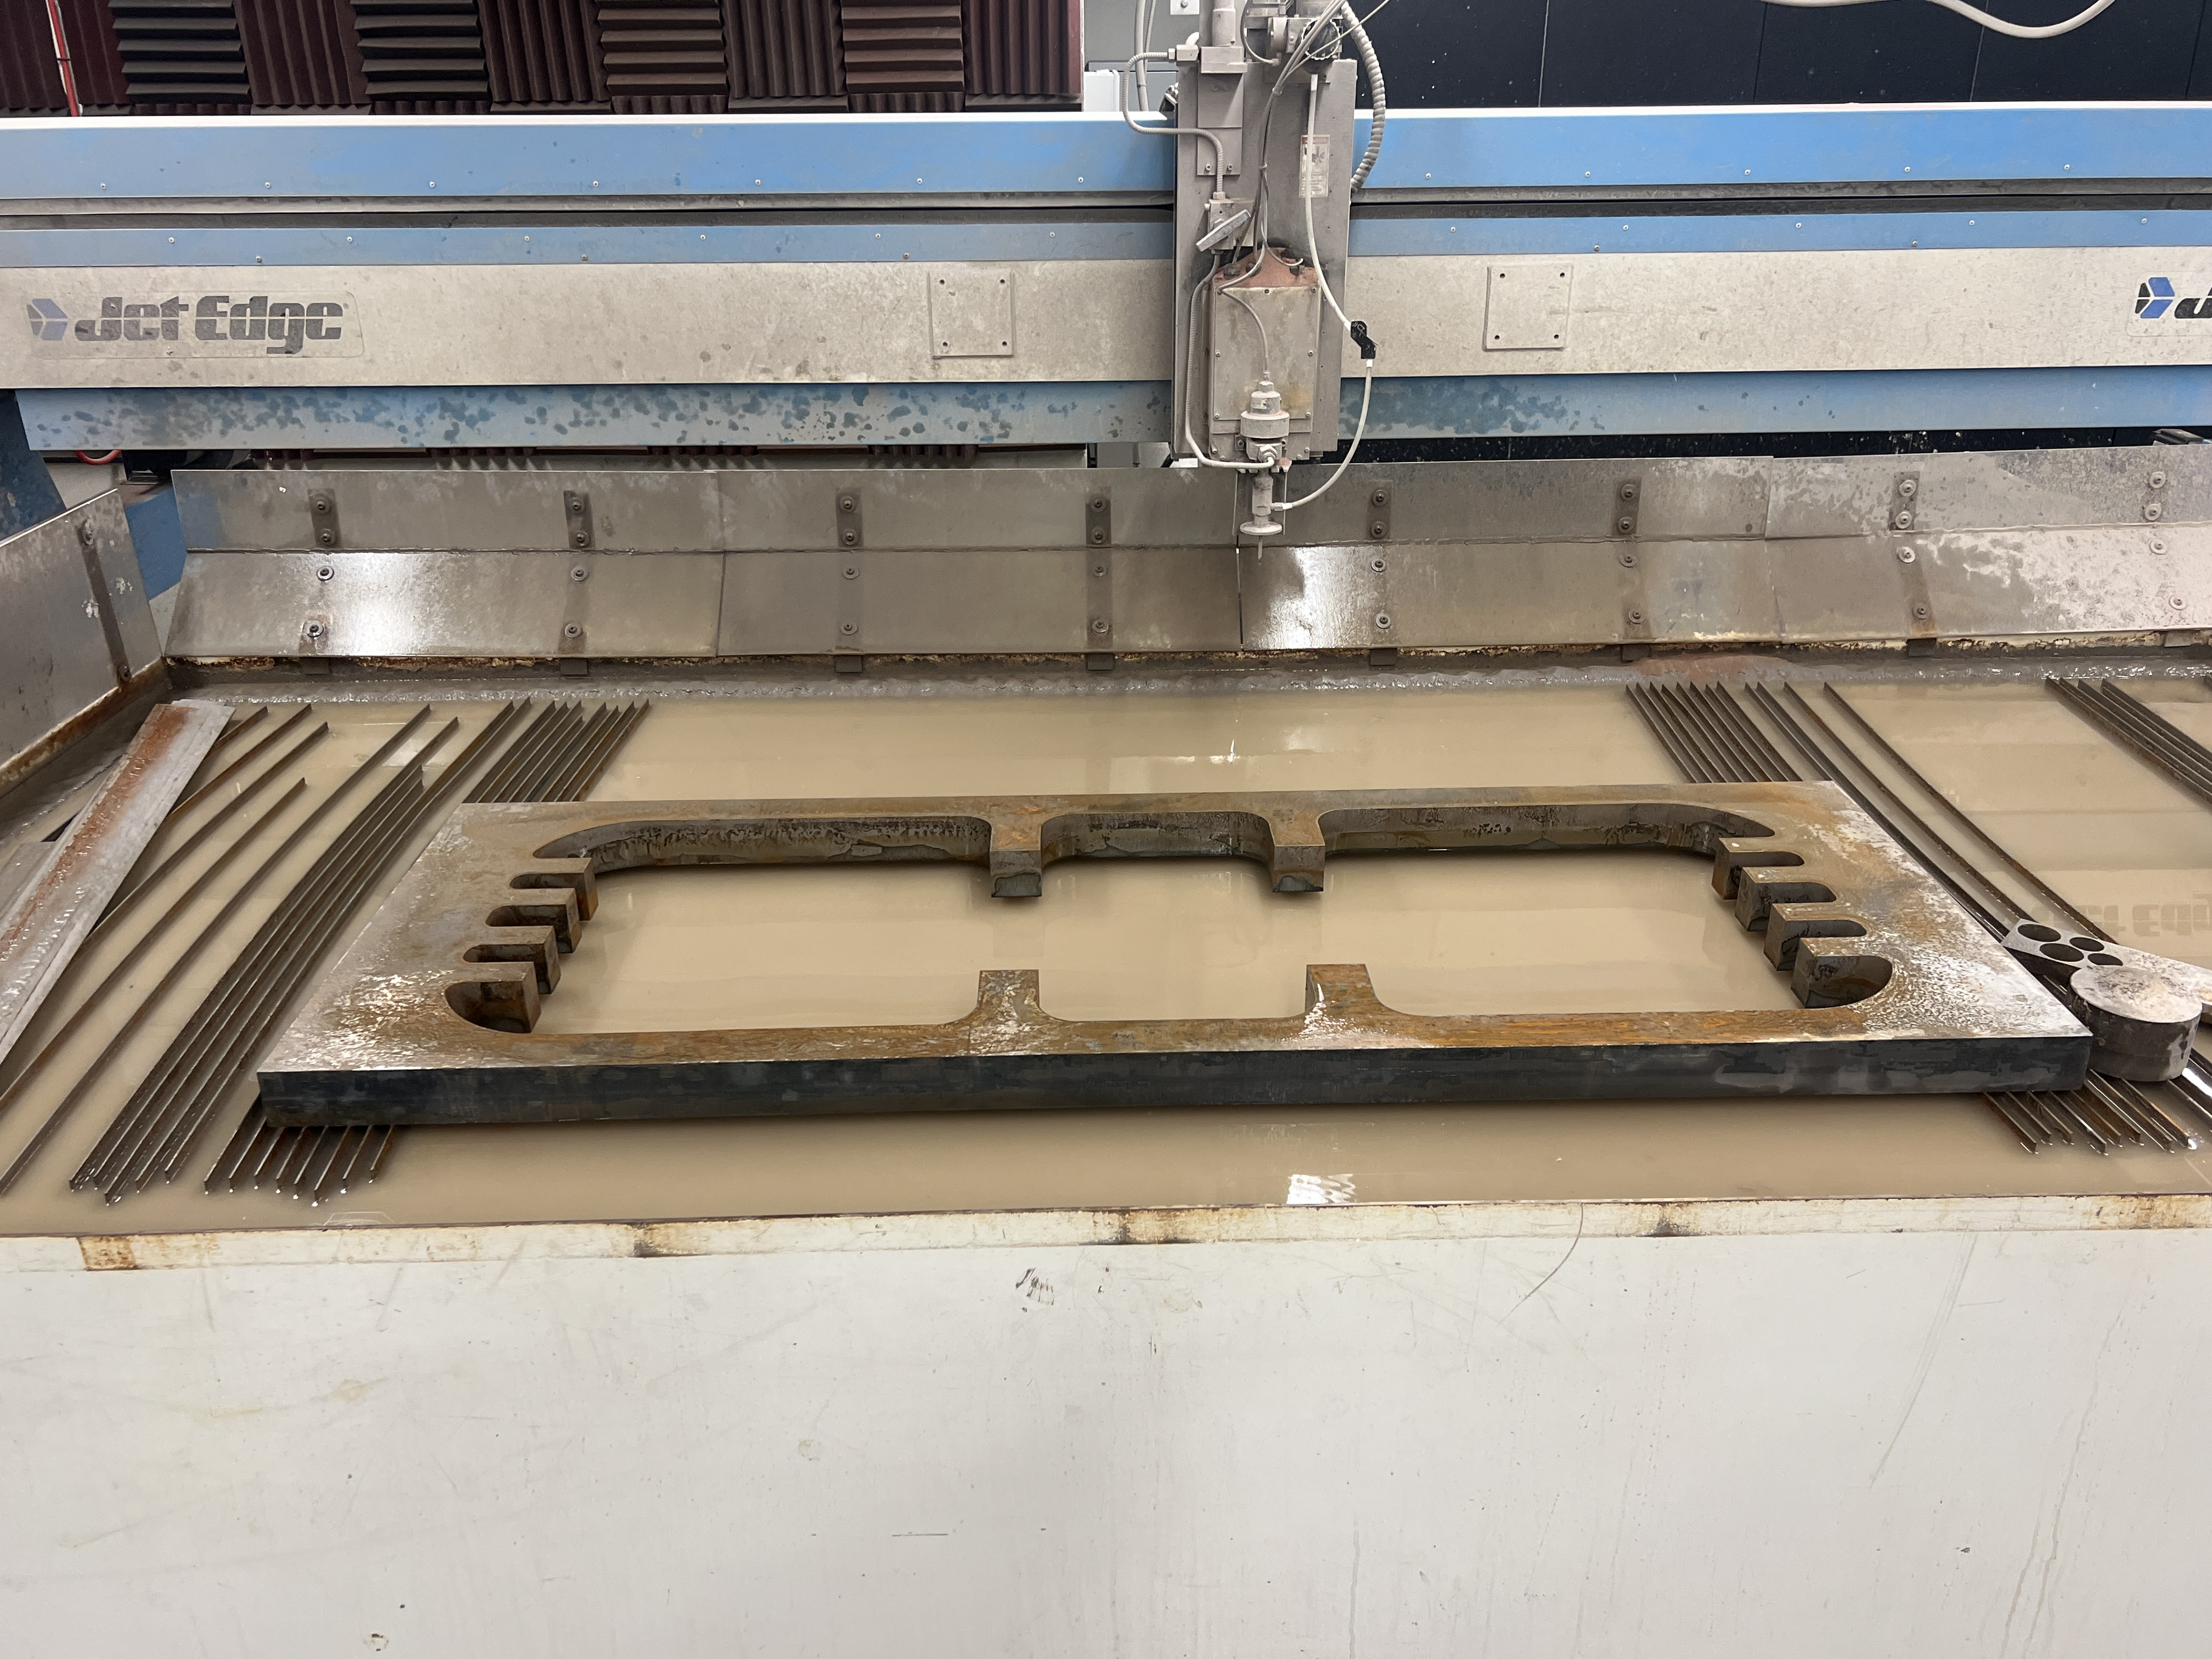
\includegraphics[width=5in]{fab-brace-jet}
    \caption{Rough cut brace on water jet}
    \label{fig:fab-brace-jet}
\end{figure}

\begin{figure}[ht!]
    \centering
    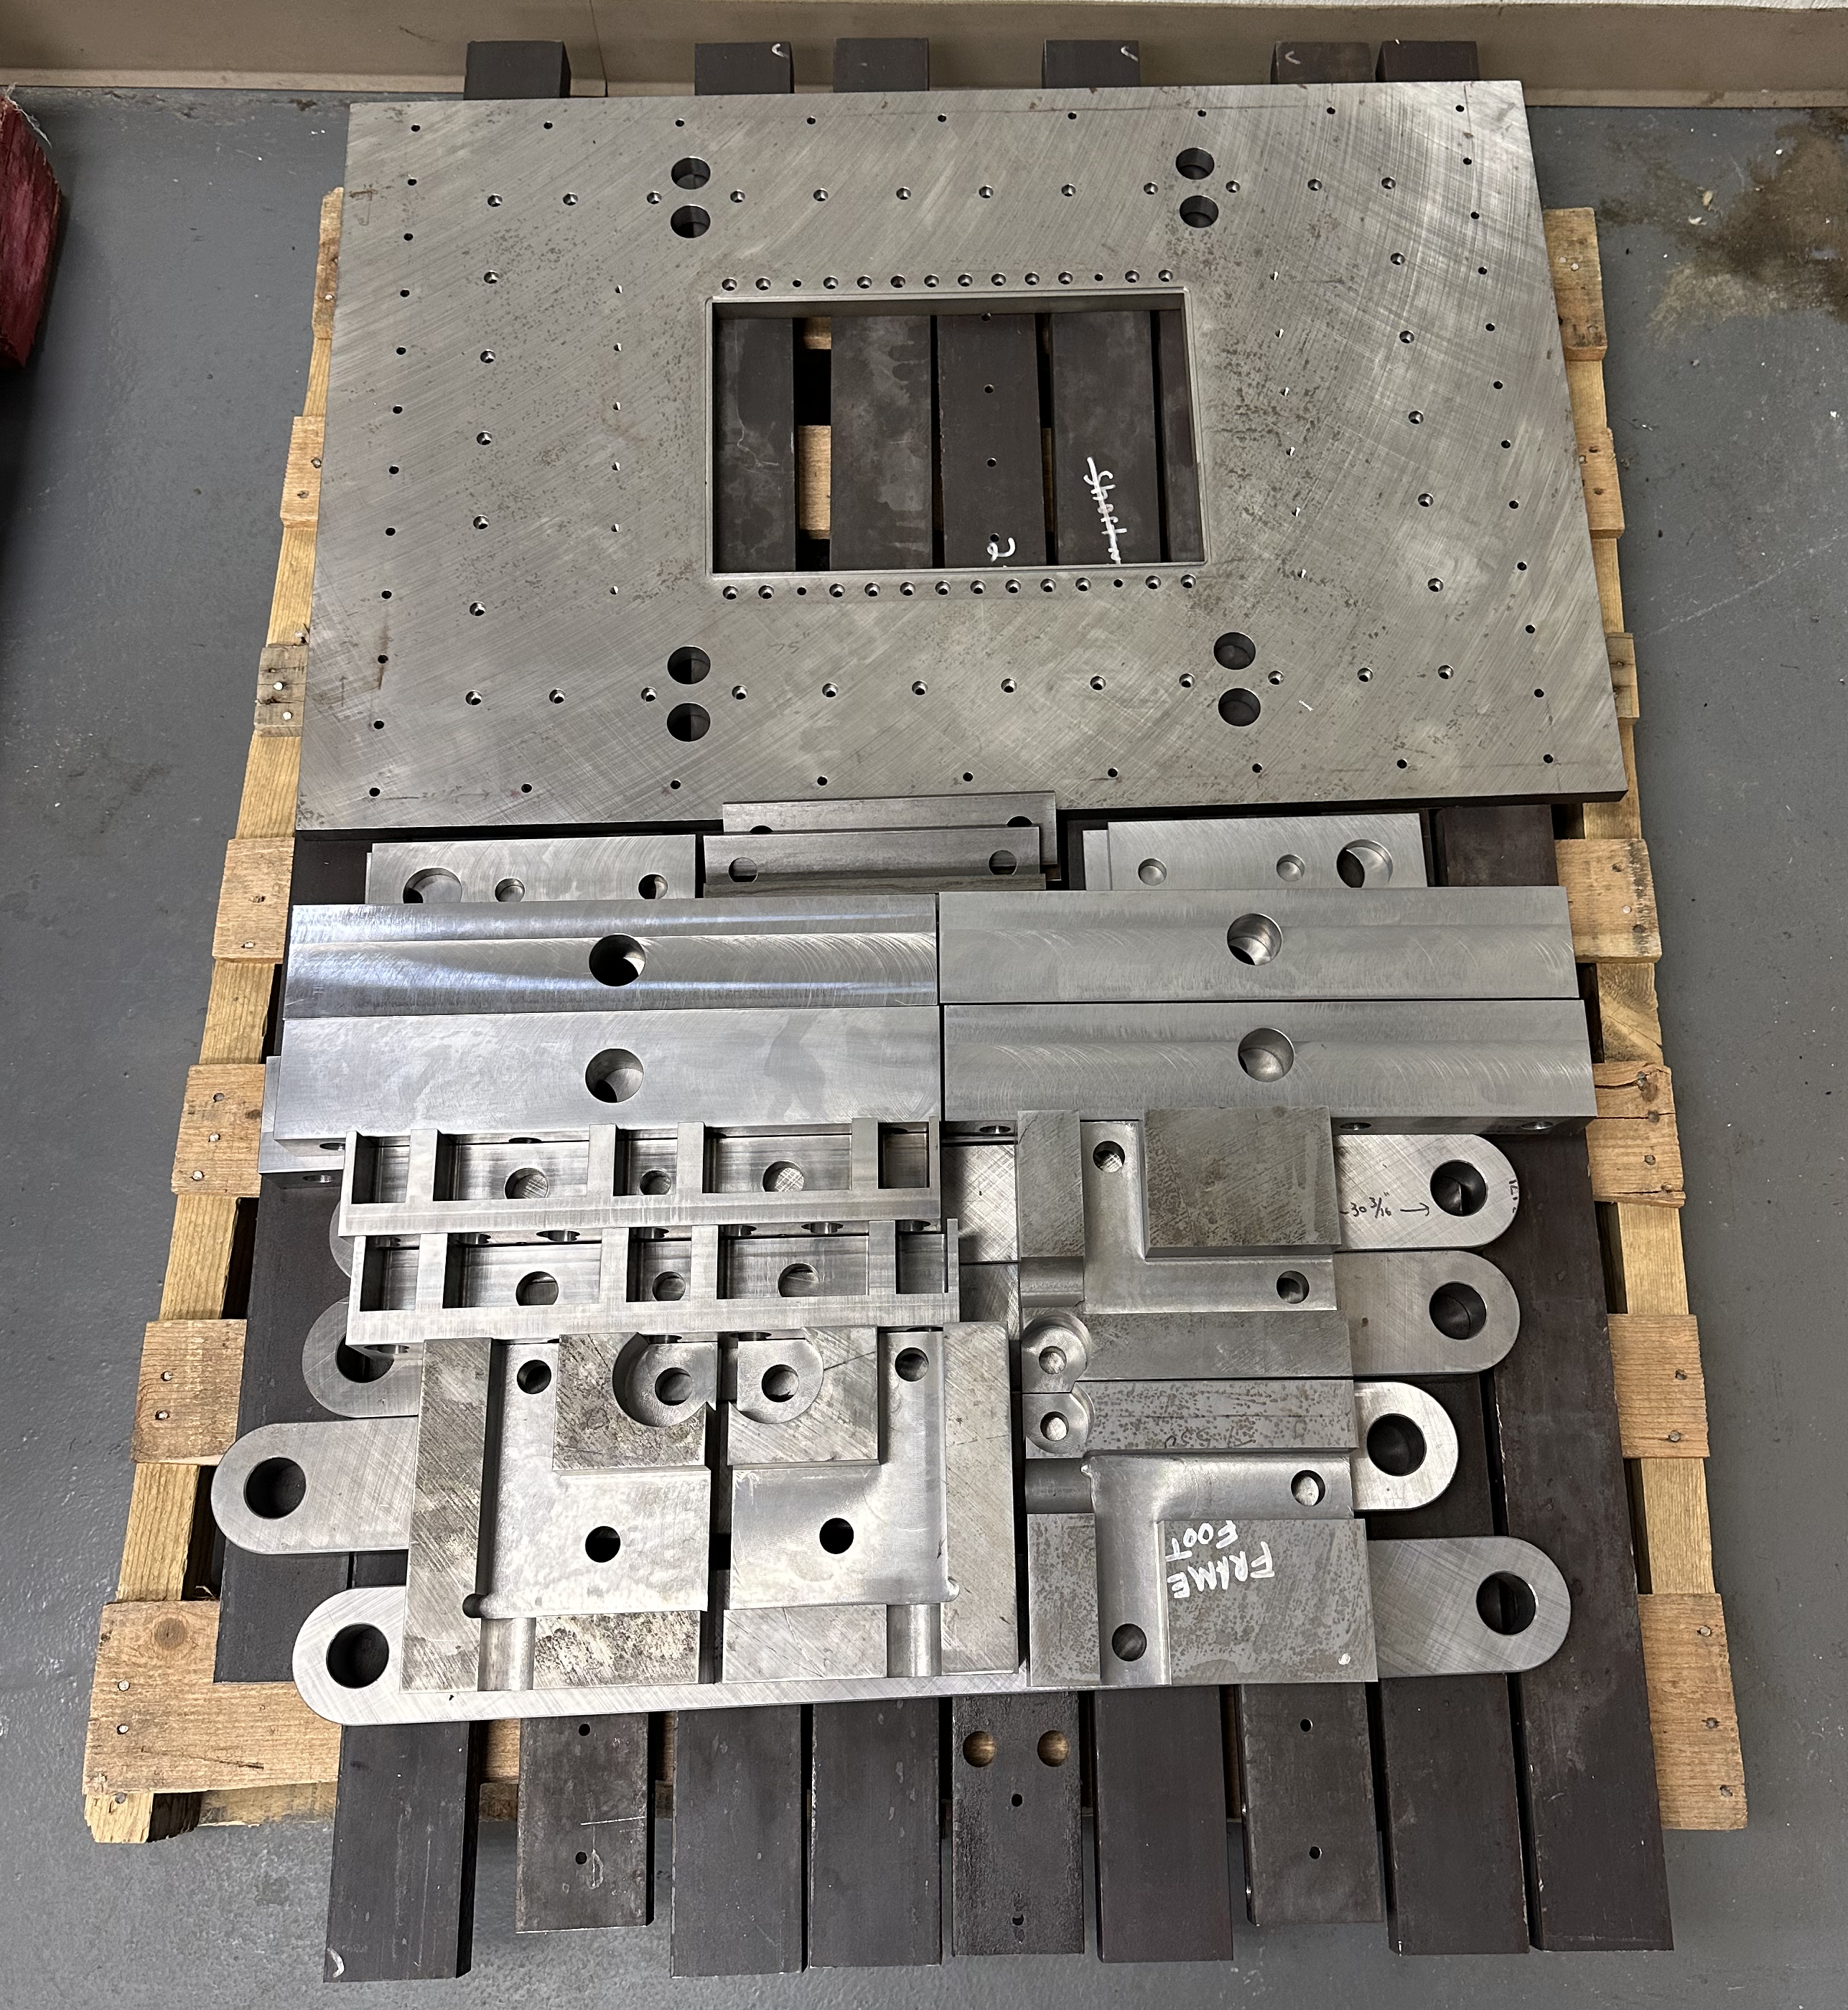
\includegraphics[width=5in]{fab-frame-parts}
    \caption{Pallet of finished frame parts from FEDC}
    \label{fig:fab-frame-parts}
\end{figure}

The nozzles and sidewalls are currently being machined at Machine Works Inc. in Bryan, TX. The nozzles were first saw cut to a rough profile to minimize the amount of time on the CNC mill, as shown in Figure \ref{fig:fab-nozzle-saw}. They are currently being machined to a rough contour, and then the back of each will be machined flat prior to finishing the contour. For the final passes, the nozzle blocks and flexures will be bolted together to ensure there is no step between the two pieces. Machine Works will also finish the brace for the frame by drilling and tapping holes.

\begin{figure}[ht!]
    \centering
    \includegraphics[width=5in]{fab-nozzle-saw}
    \caption{Nozzle block saw cut to rough profile}
    \label{fig:fab-nozzle-saw}
\end{figure}

The rest of the parts were machined at the Texas A\&M Bush Combat Development Complex (BCDC). All of these parts are finished, but only the parts necessary for the pressure test have been picked up. Figures \ref{fig:fab-flow-box}, \ref{fig:fab-aerogrid}, and \ref{fig:fab-cone} show the flow conditioner box, an aerogrid, and a flow spreading cone. BCDC will be the primary machine shop for any future fabrication throughout this work.

\begin{figure}[ht!]
    \centering
    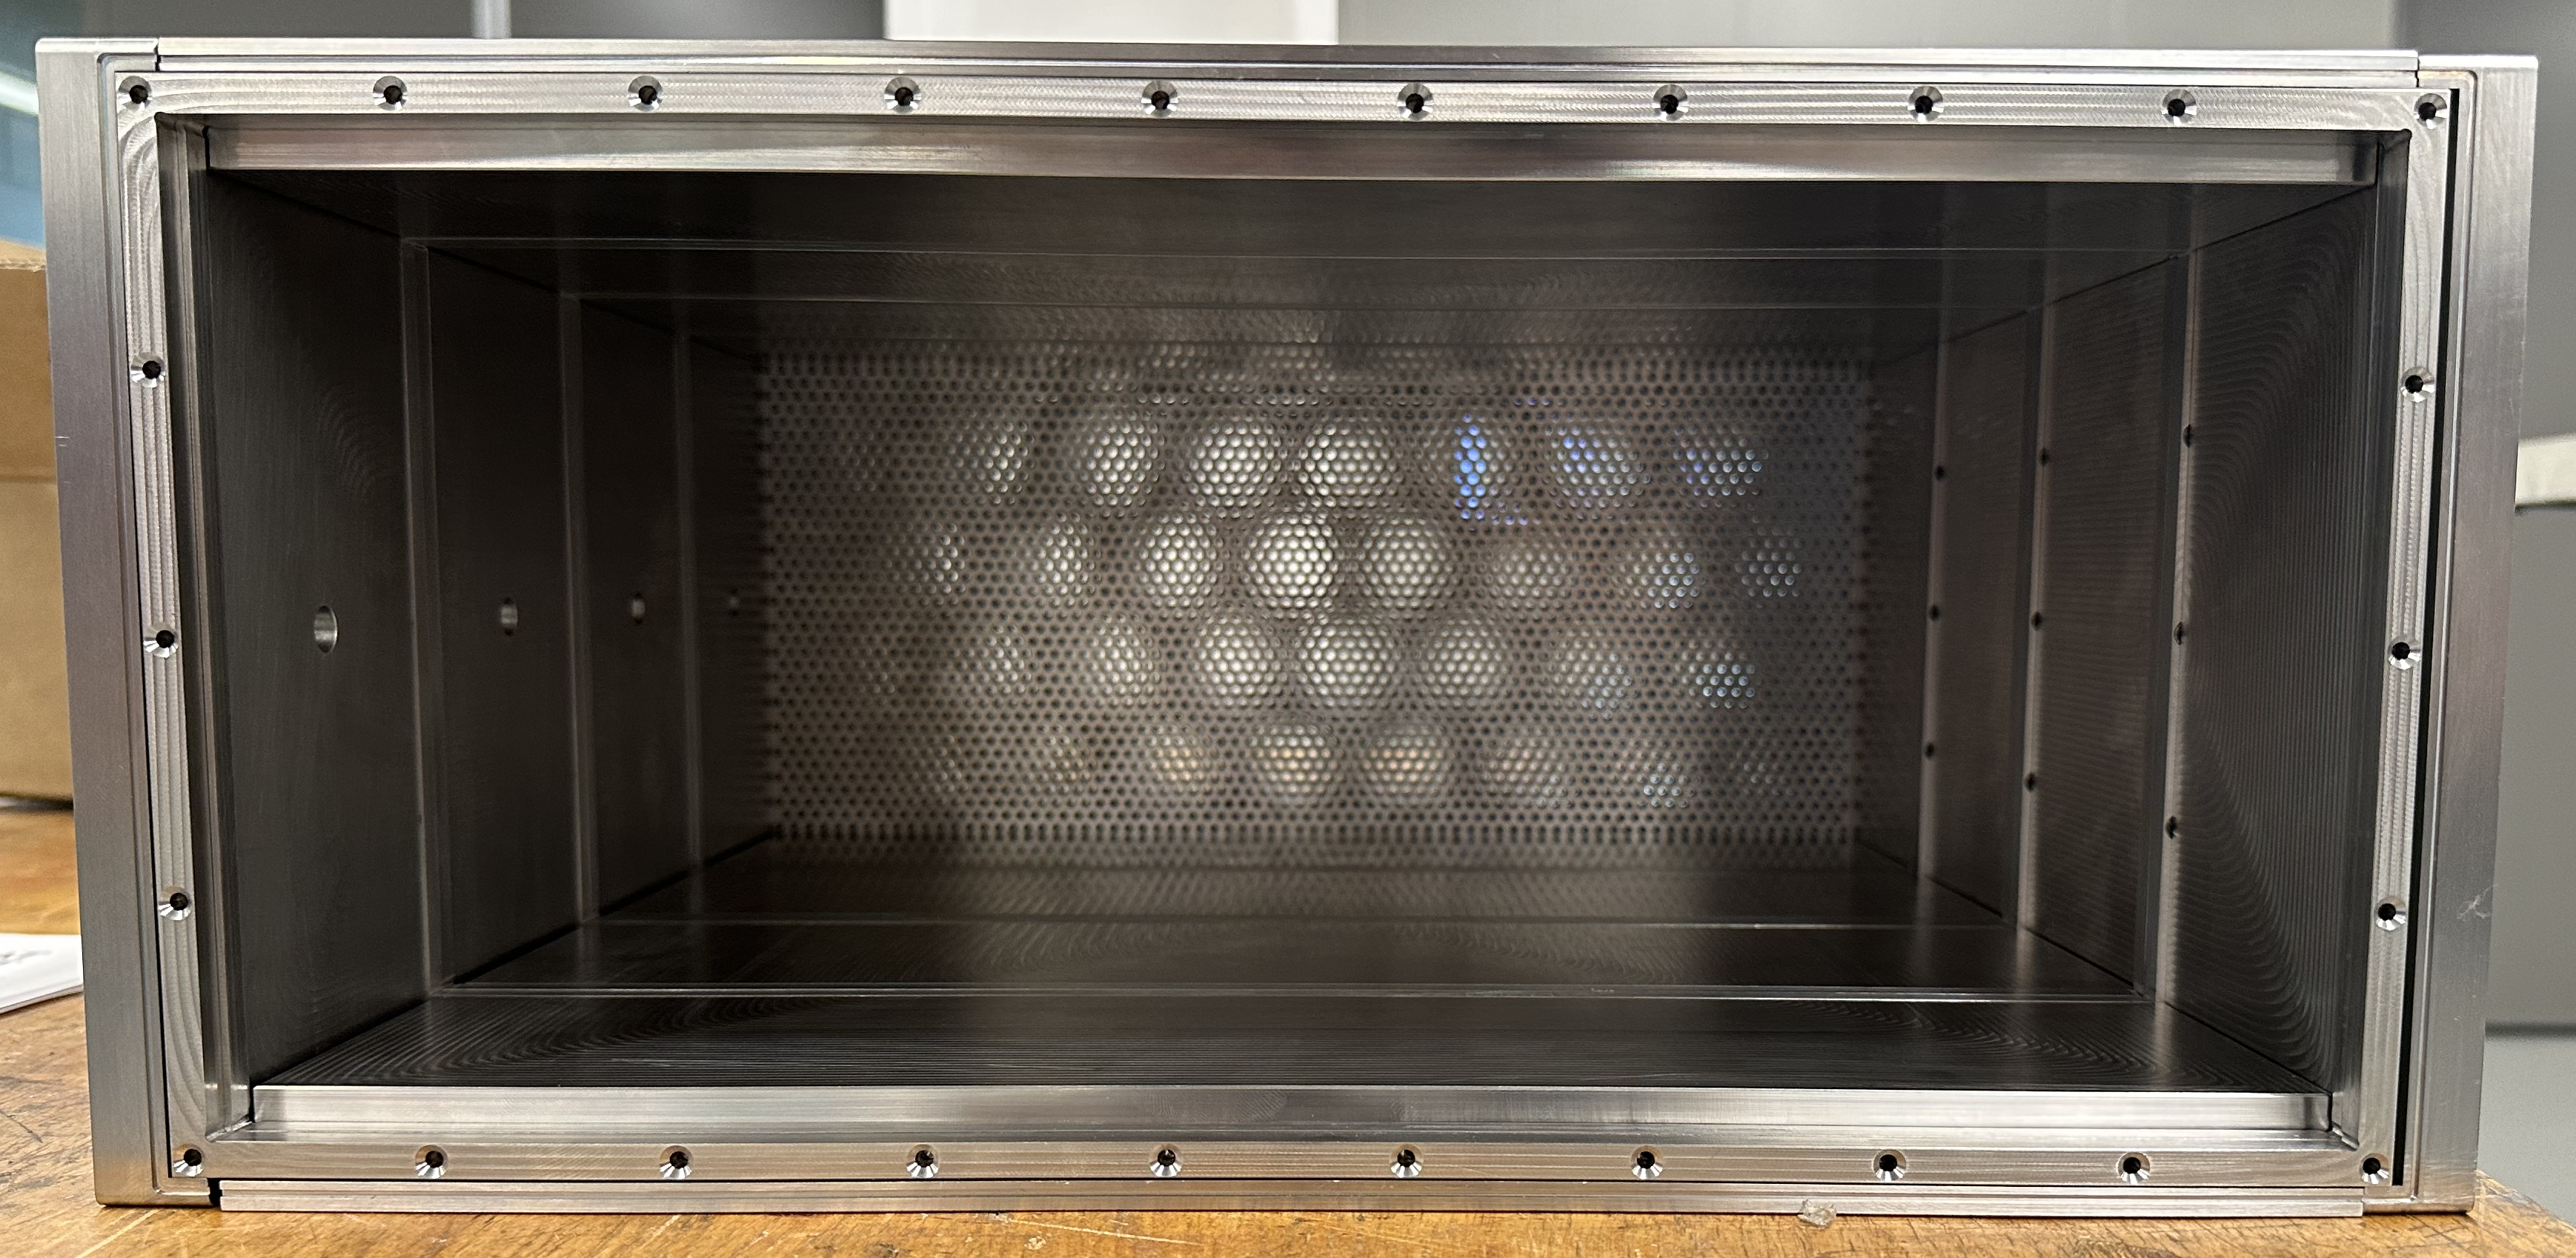
\includegraphics[width=6in]{fab-flow-box}
    \caption{Machined flow conditioner box}
    \label{fig:fab-flow-box}
\end{figure}

\begin{figure}[ht!]
    \centering
    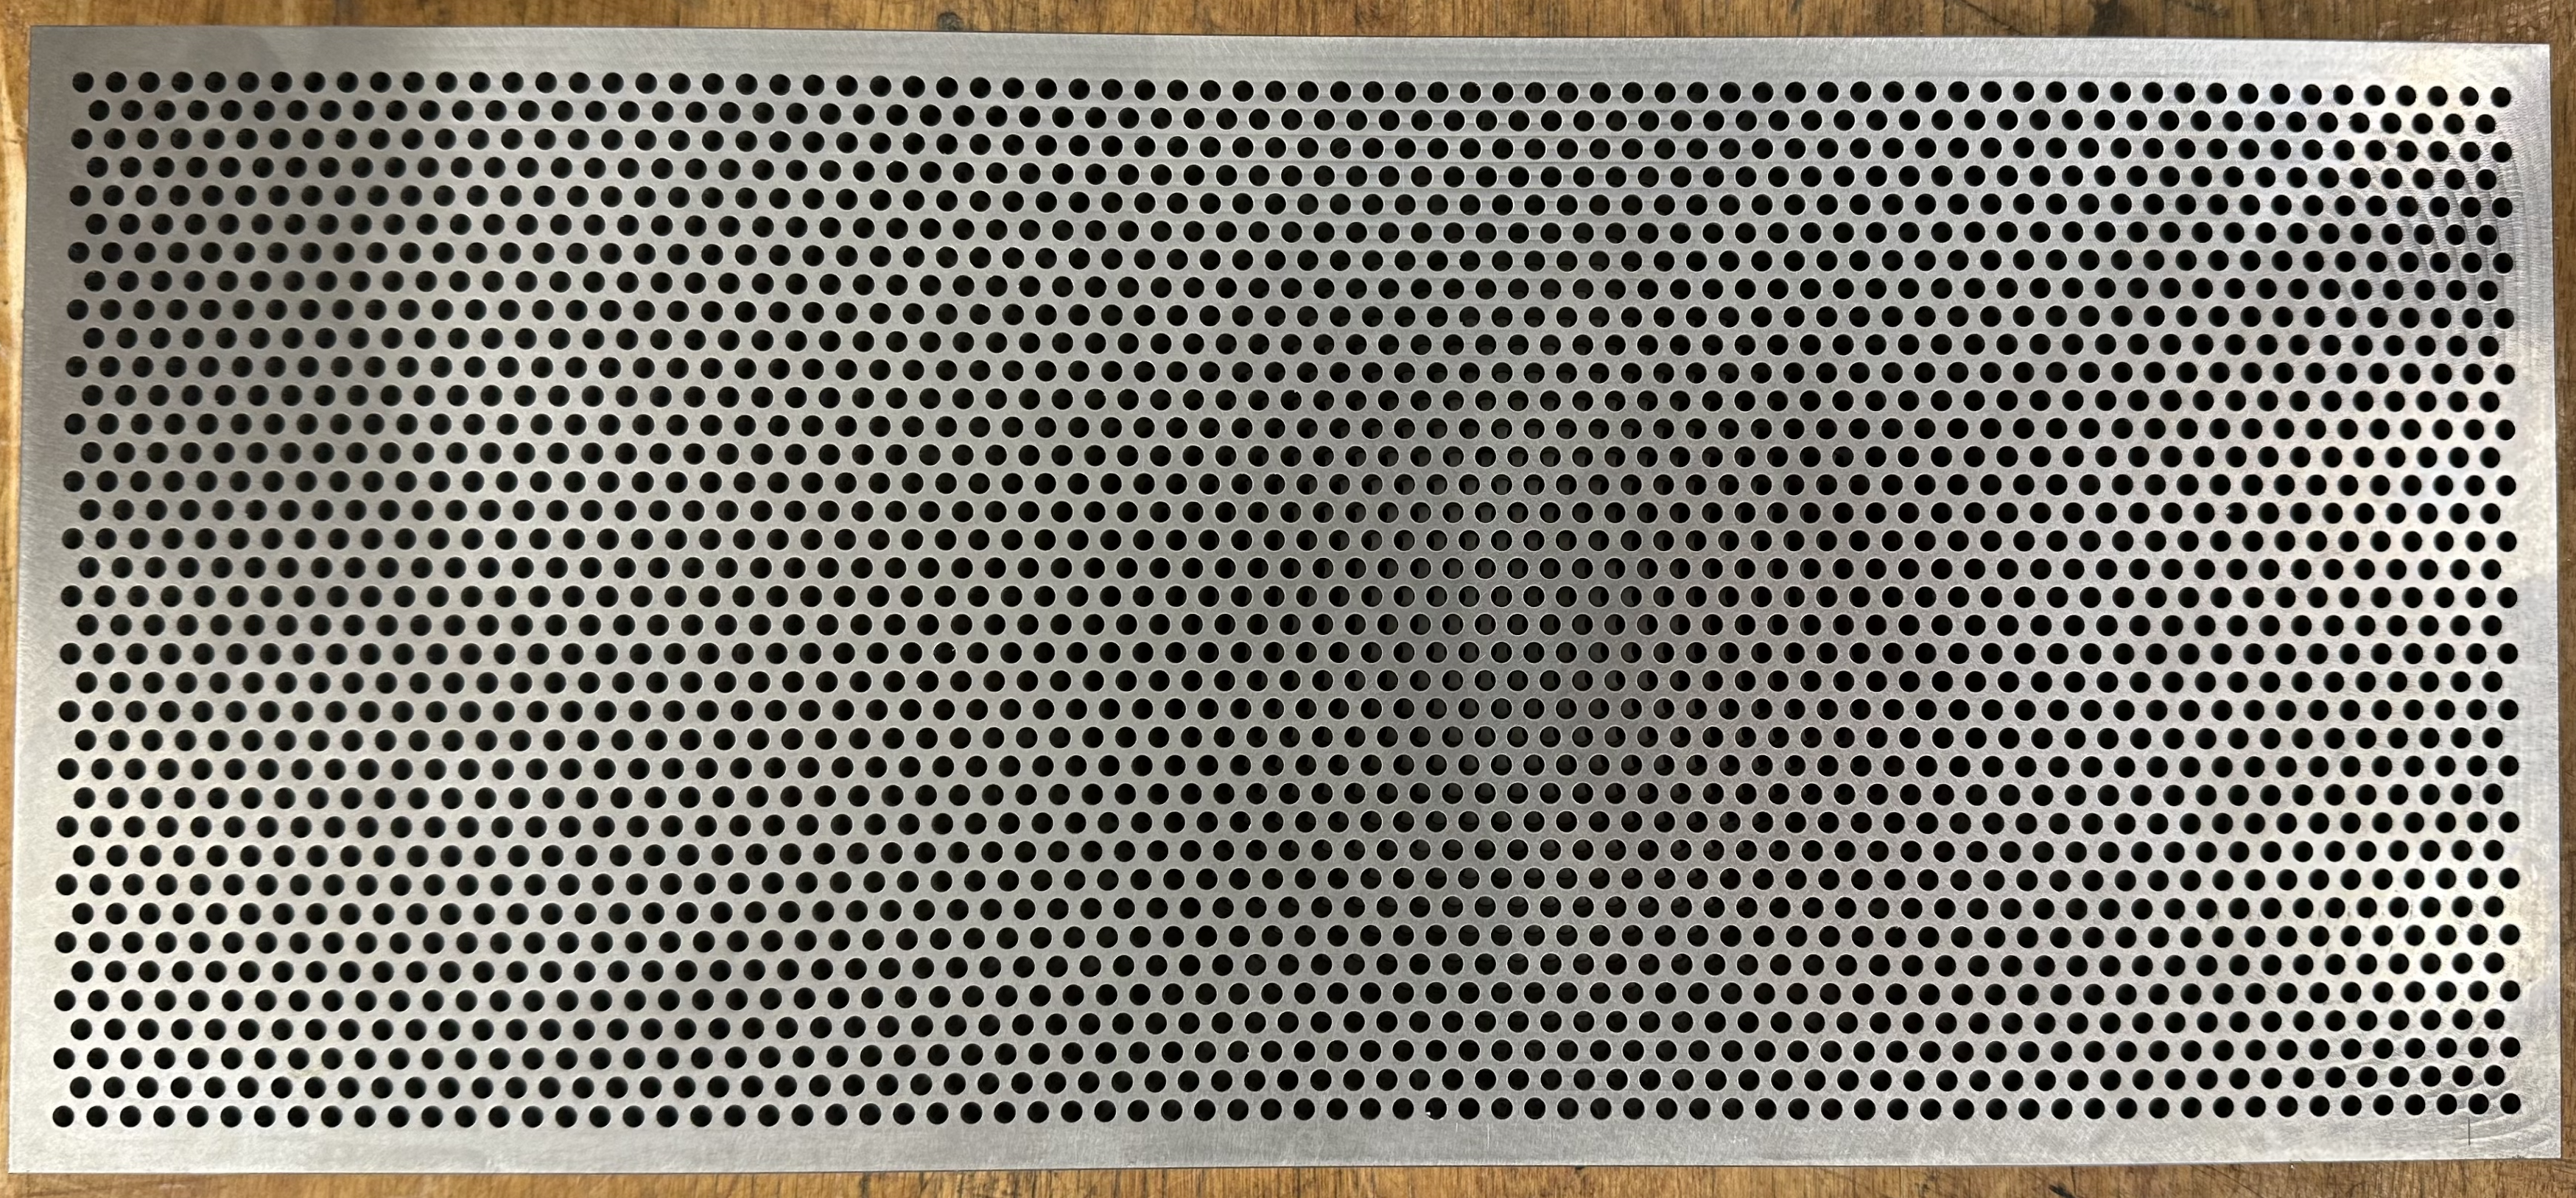
\includegraphics[width=6in]{fab-aerogrid}
    \caption{Machined aerogrid}
    \label{fig:fab-aerogrid}
\end{figure}

\begin{figure}[ht!]
    \centering
    \includegraphics[width=4in]{fab-cone}
    \caption{Machined flow spreading cone}
    \label{fig:fab-cone}
\end{figure}

\clearpage

\subsection{Pressure Test}

The hydro-pressure test will be performed at Machine Works prior to sending the nozzles and sidewalls to be polished. The base tunnel will be assembled with steel bars to simulate the actuators. The tunnel will be filled with water and pressurized to 200 psia for one hour, and the pressure will be monitored throughout. The primary goal of the pressure test is to ensure structural integrity at maximum pressure. Any major leaks will also be addressed.

\subsection{Polishing}

Following the completion of the pressure test, the nozzles and sidewalls will be shipped to Astro Pak for polishing. All interior surfaces will be mechanically polished to a 1 Ra\footnote{Surface roughness average of 1 microinch} finish, and electropolishing will be used if necessary. In order to safely ship these pieces, the nozzle blocks will be assembled as shown in Figure \ref{fig:polish-assembly} and custom wooden crates will be built.

\begin{figure}[ht!]
    \centering
    \includegraphics[trim={30 170 30 170},clip,width=5in]{polish-assembly.pdf}
    \caption{Nozzle assembly for shipping to polishing vendor}
    \label{fig:polish-assembly}
\end{figure}

\section{Final Assembly, Installation, and Calibration}

The final assembly will occur at the NAHL once the nozzle and sidewalls are delivered from polishing. Once nozzles and actuators are assembled in the frame, ACE2.0 will be rolled into the lab to replace ACE. All hoses, wires, and instrumentation attached to the nozzle and settling chamber will be removed and ACE will be rolled out of the lab. ACE2.0 will roll in and reconnect all hoses, wires, and instrumentation.

The nozzles will be leveled and aligned and then the servos will homed with the limit switches to calibrate the actuation system. The pressure and temperature instrumentation will be calibrated prior to reconnecting to the new facility. The sidewalls will then be mounted for the shakedown run, which will include a pitot rake at the nozzle exit to ensure uniformity in the test section.

% \subsection{Nozzle Alignment and Actuation Homing}

% \textcolor{red}{How to properly align and level nozzle?}

% Before the sidewalls are installed, the nozzles will be aligned and leveled and then actuated for homing the servo motors with the limit switches. At this point shims will be used to make fine adjustments to limit switch positions to ensure a minimum Mach number of \textcolor{red}{4.9?} and a maximum Mach number of \textcolor{red}{8.5?}.

% \subsection{Shakedown and Calibration}

% \textcolor{red}{Decide what the first runs and measurements should be to properly calibrate following relevant literature.}


%%%%%%%%%%%%%%%%%%%%%%%%%%%%%%%%%%%%%%%%%%%%%%%%%%%
%
%  Author: Jacob Vaughn
%  
%  Last Updated: 3/8/2024
%
%%%%%%%%%%%%%%%%%%%%%%%%%%%%%%%%%%%%%%%%%%%%%%%%%%%

%%%%%%%%%%%%%%%%%%%%%%%%%%%%%%%%%%%%%%%%%%%%%%%%%%%%%%%%%%%%%%%%%%%%%%
%%               EXPERIMENTAL SETUP
%%%%%%%%%%%%%%%%%%%%%%%%%%%%%%%%%%%%%%%%%%%%%%%%%%%%%%%%%%%%%%%%%%%%%

\chapter{EXPERIMENTAL SETUP}

Following the completed installation and calibration discussed above, each of the three primary objectives will be accomplished or demonstrated sequentially. First, the improved experimental control and efficiency as a result of the above ACE2.0 design will be demonstrated by establishing and verifying the feedback-controlled active Mach variation and selection capability as well as the Reynolds number control scheme, if implemented. Second, the freestream flow produced by the calibrated nozzle will be characterized in terms of freestream flow uniformity and disturbance levels with uncertainty quantification and an exploration hysteresis. Third, the flow parameter control capabilities will be demonstrated in a proof of concept experiment of shock interactions during a Mach trajectory and any potential hysteresis exhibited. As a result of this work, the foundation will be set for future researchers to explore dynamic hypersonic aerodynamic in a more sophisticated and efficient manner with the control capabilities of ACE2.0.

\section{Improved Experimental Control and Efficiency} 

The overall objective here is to establish and substantiate the mechanisms of ACE2.0 that allow greater control of the tunnel input parameters for both more efficient and dynamic experiments. The primary design objective of ACE2.0 was to enable active Mach number control during a run, which alone provides many key experimental advantages. However, there is still much to be desired with the parameter control capabilities to achieve full aerodynamic similarity for any flight trajectory. Thus, more precise control methods for Mach number and Reynolds number will be explored through the following objectives.

\subsection{Feedback-Controlled Active Mach Number Variation and Selection}

As stated, the primary design objective of ACE2.0 was to enable active control of the Mach number, but this capability will be taken one step further to accurately maintain the desired Mach number once set. During a tunnel run, the Mach number may vary because both pressure and thermal loads can cause the throat height to vary. Current experience shows that the Mach number can vary by up to 5\%. The goal of this work is to implement active feedback control and reduce this error to less than 0.5\%.

The general approach for this feedback control is straightforward by designing a PID controller with an input of the measured Mach number and output of actuator position or velocity. The measured Mach number is calculated from the measured stagnation pressure and static pressure by solving the isentropic relation:
\begin{equation} 
    M = \sqrt{\frac{2}{\gamma - 1} \left[\left(\frac{P_0}{P}\right)^{\frac{\gamma - 1}{\gamma}} - 1\right]}
\end{equation}

\noindent The relationship between the throat height and the Mach number is given by:
\begin{equation}
    \frac{A^*}{A} = \frac{h^*}{h_{\mathrm{exit}}} = M \left[ \left( \frac{2}{\gamma+1}  \right) \left( 1 + \frac{\gamma-1}{2} M^2  \right) \right]^{-\frac{\gamma+1}{2(\gamma-1)} }
\end{equation}

\noindent This is then subtracted from the set throat height to get the error signal for the PID transfer function:
\begin{equation}
    E(s) = h_{\mathrm{set}} - H(s)
\end{equation}

There are many design options for PID controllers depending on the desired performance characteristics. The standard approach is simply a PI controller due to the derivative action amplifying measurement noise and potential causing instability \cite{fung}. However, the derivative effect of limiting overshoot and settling time is desirable, so it will not be neglected entirely. One final option is to add high frequency filtering into the derivative term to mitigate the effects of measurement noise. Each of these options will be explored, and the following equations show the transfer functions for PI, PID, and PID with high frequency noise filtering respectively:
\begin{subequations}
    \begin{align}
        G(s) = \frac{H(s)}{E(s)} &= K \left(1 + \frac{1}{T_i s}\right) \label{eq:M-PI}\\
                                 &= K \left(1 + \frac{1}{T_i s} + T_d s\right) \label{eq:M-PID}\\
                                 &= K \left(1 + \frac{1}{T_i s} + \frac{T_d s}{1+\frac{T_d s}{N}}\right), \; N=2\textrm{ to }20 \label{eq:M-PID-filter}
    \end{align}
\end{subequations}

In practice, the Sysmac software used to write the logic for the PLC has a built-in PID function with gain autotuning capability. This will be explored in detail first in simulations in Sysmac followed by active tests in ACE2.0. This built-in PID loop will be used permanently if the resulting Mach number control is sufficient. Otherwise, the PID controller described above will be fully developed and implemented. In either case, a gain schedule will also be developed to modify the controller response throughout the Mach range to best handle the nonlinearity of the throat height and Mach number relationship.

\subsection{Reynolds Number Control Scheme}

In subscale model experiments, the Reynolds number plays an important role in maintaining similarity with real-world situations. Controlling the Reynolds number more effectively will enable more accurate and intentional experiments. The primary goal of this objective is to provide a feedback control scheme that allows the Reynolds number to be held at a set value that is either constant or dynamic. For the purposes of this discussion, any mention of the Reynolds number will be referring to the unit Reynolds number, $Re' = \frac{\rho U}{\mu}$.

The main control parameter for Reynolds number will be the settling chamber stagnation pressure. The Reynolds number is coupled with respect to pressure, temperature, and Mach number. The goal will be to control the stagnation pressure to counteract changes in both temperature and Mach number. For reference, the settling chamber stagnation temperature typically increases during a run by up to 40 K, and, of course, the Mach number can vary between 5 and 8. The effect of temperature will be examined during both simulations and experiments to determine if a more adequate control system is required to maintain constant temperature or if this effect on the Reynolds number can be compensated by changing the pressure.

A mathematical model will be developed to be implemented for future physical PID control of the pressure regulator and the Reynolds number as a result. The physical implementation of this controller in this work will be dependent on budget and schedule constraints. The primary constraint here will be the ability to quickly replace the existing regulator manual valve control with a controlled valve. The M6QT utilizes the same air supply infrastructure, so any complications throughout the valve replacement process would result in both facilities being inoperable and a delay in all planned research for this work and others.

One other factor to be considered in the stagnation pressure control is the time response delay due to both the distance between the regulator and the tunnel and the maximum operating speed of the regulator. The distance from the regulator to the settling chamber inlet is around 25 feet, resulting in a maximum response time in the range 20 to 150 milliseconds. This range  considers the minimum sound speed of $a = \sqrt{\gamma R T_0} = 3.28\sqrt{(1.4)(287)(300)} \approx 1140 \; \frac{ft}{s}$ for the pressure waves and the minimum pipe flow velocity of $v_{pipe,min} = \dot{m}_{min}/\rho/A_{pipe} \approx 164 \; \frac{ft}{s}$ for the corresponding mass flow to reach the settling chamber. The full response time cannot be calculated currently because the maximum regulator operating speed is unknown. With this in mind, the response time will be investigated experimentally if the Reynolds number control is implemented in this work.

The following derivation provides a starting point for the mathematical model. 

\begin{equation}
    \frac{T_0}{T} = (1+\frac{\gamma-1}{2}M^2) = F
\end{equation}
\begin{equation}
    \frac{P_0}{P} = (1+\frac{\gamma-1}{2}M^2)^{\frac{\gamma}{\gamma+1}} = F^{\frac{\gamma}{\gamma+1}}
\end{equation}
\begin{equation}
    \rho = \frac{P}{R T} = \frac{P_0 F^{\frac{-\gamma}{\gamma-1}}}{R T_0 F^{-1}} = \frac{P_0}{R T_0 F^{\frac{1}{\gamma-1}}}
\end{equation}
\begin{equation}
    U = M \sqrt{\gamma R T} = M F^{-\frac{1}{2}} \sqrt{\gamma R T_0}
\end{equation}
\begin{equation*}
    Re' = \frac{\rho U}{\mu} = \frac{1}{\mu} \frac{P_0}{R T_0 F^{\frac{1}{\gamma-1}}} M F^{-\frac{1}{2}} \sqrt{\gamma R T_0}
\end{equation*}
\begin{equation}
    Re' = \sqrt{\frac{\gamma}{R T_0}} \frac{M P_0}{\mu} F^{-\frac{\gamma+1}{2(\gamma -1}}
\end{equation}


\noindent Differentiating $Re'$ assuming $\gamma$ and $R$ are constant and with $\frac{dF}{dt} = (\gamma-1)M \frac{dM}{dt}$ gives:
\begin{equation}
    \frac{d(Re')}{dt} = \sqrt{\frac{\gamma}{R T_0}} \frac{M P_0}{\mu} F^{-\frac{\gamma+1}{2(\gamma -1}} \left[ \frac{\frac{dM}{dt}}{M} + \frac{\frac{dP_0}{dt}}{P_0} - \frac{\frac{dT_0}{dt}}{2T_0} - \frac{\frac{d\mu}{dt}}{\mu} - \frac{\gamma+1}{2} M F^{-1} \frac{dM}{dt} \right]
\end{equation}

\noindent With $\mu$ defined from Sutherland's Law with $T_\mu = 273$, $S_\mu = 111$, and $\mu_0 = 1.716 \times 10^{-5}$:
\begin{equation}
    \mu = \mu_0 \frac{T_\mu+S_\mu}{T+S_\mu} \left( \frac{T}{T_\mu} \right)^{\frac{3}{2}}
\end{equation}
\begin{equation}
    \mu = \frac{\mu_0(T_\mu+S_\mu)}{T_\mu^{\frac{3}{2}}} \frac{T_0^{\frac{3}{2}} F^{-\frac{3}{2}}}{T_0 F^{-1}+S_\mu}
\end{equation}

Following the same logic as before, either a PI, PID, or PID with high frequency noise filtering will be implemented based on experimental results of Reynolds number control. However, in this case the calculated Reynolds number will be subtracted from the set condition to get the error signal and the controlled parameter will either be the stagnation pressure or the respective regulator position.
\begin{equation}
    E(s) = Re'_{\mathrm{set}} - Re'(s)
\end{equation}

\vspace{-1.5cm}
\begin{subequations}
    \begin{align}
        G(s) = \frac{P_0(s)}{E(s)} \textrm{ or } \frac{X(s)}{E(s)} &= K \left(1 + \frac{1}{T_i s}\right) \label{eq:Re-PI}\\
                                 &= K \left(1 + \frac{1}{T_i s} + T_d s\right) \label{eq:Re-PID}\\
                                 &= K \left(1 + \frac{1}{T_i s} + \frac{T_d s}{1+\frac{T_d s}{N}}\right), \; N=2\textrm{ to }20 \label{eq:Re-PID-filter}
    \end{align}
\end{subequations}

At the very least, this model will be fully developed and simulated to ensure minimal future work for implementation. The physical control mechanism will also be explored and potentially purchased to allow install at the earliest convenience between the ACE2.0 and M6QT schedules.

\section{Freestream Flow Uniformity and Disturbance Levels Characterization}

In order to establish a baseline of performance characteristics for future work within the ACE2.0 facility, a pitot and hot-wire survey will be performed to measure and characterize the freestream flow uniformity and disturbance levels (noise) throughout the nozzle. The survey will utilize both a pitot rake and a single pitot probe with Kulite pressure transducers mounted on a traverse to characterize the pressure fluctuations and uniformity and a hot-wire anemometer to measure mass flux fluctuation levels.

A final noise survey was performed in ACE to establish a control for comparison with ACE2.0 as well as provide a preliminary exploration of noise hysteresis. The survey utilized a single pitot probe to measure the noise along the centerline at 6 and 24 inches upstream of the nozzle exit as shown in Figure \ref{fig:pitot17}. For each run, the Reynolds number was increased above the transition value $\left(Re' = 3 \times 10^6/\mathrm{m}\right)$ discussed in the previous chapter and then decreased back down to the initial value below the transition value. These measurements provided baseline data for pressure fluctuation hysteresis. The results are shown in Figure \ref{fig:ace-hysteresis}. As seen, there is some discernible hysteresis in the freestream pressure fluctuation levels as the Reynolds number is swept up and back down. This survey will be repeated using a hot-wire anemometer to measure mass flux fluctuation levels if the remaining schedule for ACE permits.

\begin{figure}[ht!]
    \centering
    \includegraphics[width=6in]{ace-hysteresis}
    \caption{ACE freestream pressure fluctuations at 6 inches and 24 inches upstream of nozzle exit}
    \label{fig:ace-hysteresis}
\end{figure}

The anticipated characterization test matrix for ACE2.0 is shown in Table \ref{tab:ace2-survey}. The pitot rake will be used to characterize the freestream flow uniformity in the nozzle exit plane and a plane 6 inches upstream. The single pitot probe and hot-wire anemometer will be used to measure the freestream pressure fluctuation and mass flux fluctuation levels, respectively, along the centerline up to 24 inches upstream of the nozzle exit. The runs in each test matrix are divided into a few distinct objectives: (1) uniformity, (2) uncertainty quantification, (3) disturbance levels transition, and (4) hysteresis. The last five runs will be replicates of the first five to better quantify the uncertainty in Mach number, Reynolds number, and flow uniformity. This entire process will be documented so that flow-quality verification tests can be repeated as part of ongoing lab operations.

\begin{figure}[ht!]
    \centering
    \includegraphics[width=6in]{pitot17}
    \caption{Pitot probe measuring 24 inches upstream of nozzle exit}
    \label{fig:pitot17}
\end{figure}

\setcounter{rownum}{0}
\begin{table}[ht!]
    \centering
    \begin{tabular}{|>{\stepcounter{rownum}\therownum}c|c|c|c|c|c|c|c|}
        \hline
        \multicolumn{1}{|c|}{\textbf{Run}} & \textbf{X (in.)} & \textbf{Y (in.)} & \textbf{Z (in.)} & \textbf{Mach} & \textbf{$Re'$ ($10^6$)} & \textbf{ Instrument} & \textbf{Purpose} \\ \hline
        & 0 & -3:1:3 & 0 & 6$^*$ & 3$^*$ & Rake & Uniformity\\ \hline
        & 0 & -3:1:3 & -3:1:3 & 8 & 3 & Rake & Uniformity\\ \hline
        & 0 & -3:1:3 & -3:1:3 & 7 & 3 & Rake & Uniformity\\ \hline
        & 0 & -3:1:3 & -3:1:3 & 6 & 3 & Rake & Uniformity\\ \hline
        & 0 & -3:1:3 & -3:1:3 & 5 & 3 & Rake & Uniformity\\ \hline
        & -6 & -3:1:3 & -3:1:3 & 5 & 3 & Rake & Uniformity\\ \hline
        & -6 & -3:1:3 & -3:1:3 & 6 & 3 & Rake & Uniformity\\ \hline
        & -6 & -3:1:3 & -3:1:3 & 7 & 3 & Rake & Uniformity\\ \hline
        & -6 & -3:1:3 & -3:1:3 & 8 & 3 & Rake & Uniformity\\ \hline
        & 0 & 0 & 0 & 8 & 2$\to$7$\to$2 & Pitot & Noise\\ \hline
        & 0 & 0 & 0 & 7 & 2$\to$7$\to$2 & Pitot & Noise\\ \hline
        & 0 & 0 & 0 & 6 & 2$\to$7$\to$2 & Pitot & Noise\\ \hline
        & 0 & 0 & 0 & 5 & 2$\to$7$\to$2 & Pitot & Noise\\ \hline
        & 0 & 0 & 0 & 5$\to$8$\to$5 & 3 & Pitot & Noise\\ \hline
        & -6 & 0 & 0 & 5$\to$8$\to$5 & 3 & Pitot & Noise\\ \hline
        & -6 & 0 & 0 & 5 & 2$\to$7$\to$2 & Pitot & Noise\\ \hline
        & -6 & 0 & 0 & 6 & 2$\to$7$\to$2 & Pitot & Noise\\ \hline
        & -6 & 0 & 0 & 7 & 2$\to$7$\to$2 & Pitot & Noise\\ \hline
        & -6 & 0 & 0 & 8 & 2$\to$7$\to$2 & Pitot & Noise\\ \hline
        & -17 & 0 & 0 & 6 & 2$\to$7$\to$2 & Pitot & Noise\\ \hline
        & -17 & 0 & 0 & 5$\to$8$\to$5 & 3 & Pitot & Noise\\ \hline
        & -24 & 0 & 0 & 5$\to$8$\to$5 & 3 & Pitot & Noise\\ \hline
        & -24 & 0 & 0 & 6 & 2$\to$7$\to$2 & Pitot & Noise\\ \hline
        -\stepcounter{rownum}\stepcounter{rownum}\stepcounter{rownum}\stepcounter{rownum}\stepcounter{rownum}\stepcounter{rownum}\stepcounter{rownum}\stepcounter{rownum}\stepcounter{rownum}\stepcounter{rownum}\stepcounter{rownum}\stepcounter{rownum}\stepcounter{rownum}\therownum & \multicolumn{6}{|c|}{\textbf{Repeat runs 10-23 with Hot-wire}} & Noise\\ \hline
        -\stepcounter{rownum}\stepcounter{rownum}\stepcounter{rownum}\stepcounter{rownum}\therownum & \multicolumn{6}{|c|}{\textbf{Replicate runs 1-5}} & Uncertainty\\ \hline
    \end{tabular}
    \caption{Test matrix for ACE2.0 freestream characterization.}
    \label{tab:ace2-survey}
\end{table}

\subsection{Freestream Uncertainty Quantification}

The process to quantify the uncertainty of the various parameters for this work will closely follow Stephens's et al. \cite{stephens-hubbard} and Curriston's \cite{curriston-dis} approaches by simply focusing on establishing a baseline for the uncertainty and making recommendations for improvement if necessary. The three steps to establish this baseline uncertainty for ACE2.0 will be (1) gather/measure systematic elemental uncertainties, (2) input into a Monte Carlo code along with data reduction equations to simulate systematic uncertainties, and (3) measure repeat data points through a few replicate experiments and calculate random uncertainties.

First, the systematic elemental uncertainties can be gathered and measured from the various sensors, which includes the static pressure transducer, stagnation pressure transducer, stagnation temperature thermocouple, and servo motor internal encoders. Each of these has a predefined manufacturer uncertainty that can be used, but some of these are very conservative and not ideal. The pressure sensors and temperature sensor will be tested against a working standard to measure the true uncertainty, which is often found to be an order of magnitude less than the manufacturer uncertainty \cite{curriston-dis}. The systematic uncertainly of any sensors utilized in future experiments is outside the scope of this work and must be considered when calculating the total uncertainty of measurements in each experiment.

Next, these systematic elemental uncertainties will be propagated through a Monte Carlo simulation along with the specific data reduction equations for the facility. This output will provide the total systematic uncertainty for each parameter of interest, which will be added to the random uncertainty to give the total uncertainty. Additionally, this simulation will also be used provide a sensitivity analysis of the uncertainty to the various input parameters. This will be insightful on how to best improve the uncertainty if necessary.

Finally, repeat data points will be measured by repeatedly settling on and off the set condition for the parameter of interest. While data will be gathered throughout the entire characterization test matrix, runs 1 and 20 will be solely for repeat data measurements. These two runs will provide a direct comparison of replicates that will account for any correlations that were not considered or unquantifiable. The standard deviation of this data will be added in quadrature to the systematic uncertainty to calculate the total uncertainty for each parameter of interest for the freestream flow.

\subsection{Freestream Disturbance Hysteresis}

Dynamic sweeps of both Mach number and Reynolds number will be performed to explore any potential hysteresis effects in either the noise or the control parameters. Specifically, this will be accomplished during the dynamic runs in the characterization test matrix in Table \ref{tab:ace2-survey}. The goal is simply to identify the existence of any hysteresis effects to inform future work within ACE2.0. The Reynolds number sweep runs are necessary to determine the value at which transition occurs, so sweeping the Reynolds number back down will not add any additional work and will be ensure that there is no hysteresis. For the Mach number however, there is no past data to determine the existence of hysteresis, so these runs will establish a baseline. The noise level is known to decrease with an increase in Mach number, so identifying any hysteresis in this will be necessary to inform future experiments.

\section{Mach Trajectory and Potential Hysteresis Proof of Concept Experiment}

This objective will primarily serve as a demonstration of the capabilities for ACE2.0 and will also provide preliminary insight into the hysteretic behavior of dynamic Mach number experiments. The flow characteristic that will be specifically explored in this research will be shock interactions using schlieren. The goal will be to observe hysteresis in the transition from regular reflection to Mach reflection by varying the Mach number. The challenge of this is that the only facilities that have successfully produced this hysteresis had low freestream disturbance levels and an open-jet test section, while ACE2.0 has a closed test section and is not considered a "quiet" facility. In order to provide the best conditions for hysteresis to be observed, these experiments will be performed at higher Mach numbers and a lower unit Reynolds number where freestream disturbance levels are lowest.

The experiments will be based on the methodologies and results from Durand et al. \cite{durand} and Tao et al. \cite{tao} in addition to the experimental setup of Mai \cite{mai-dis}. The Mach number will be varied across either the Von Neumann condition or the detachments criteria to force the transition from regular reflection to Mach reflection or vice versa. In order to choose the wedge angle and Mach number range for each experiment, Figure \ref{fig:dual} was created following the processes shown by Mouton \cite{mouton} for each condition. Using the pressure ratio and flow deflection angle for an oblique shock, the shock angle is solved numerically as a function of the freestream Mach number for each condition. The shock angle and Mach number are then used to produce the detachment and Von Neumann condition relationship between wedge angle and Mach number. Below the Von Neumann condition, only regular reflections are possible as shown in Figure \ref{fig:von-neumann}. Above the detachment condition, only Mach reflections are possible as shown in Figure \ref{fig:detachment}. Between these two condition, either shock formation is possible.

% The basic parameters across an oblique shock shown in Figure \ref{fig:detachment} are given as a function of the Mach number in region x $\left(M_x\right)$, the shock angle ($\alpha$), and the ratio of specific heats ($\gamma$). 

% The pressure ratio is 
% \begin{equation}
%     \xi \left(M_x,\alpha\right) = \frac{P}{P_x} = \frac{2 \gamma M_x^2 \sin^2{\alpha} - (\gamma-1)}{\gamma+1}
% \end{equation}

% \noindent The flow deflection angle (wedge angle) and Mach number are given as
% \begin{equation}
%     \theta \left(M_x,\alpha\right) = \cot^{-1}{\left[ \left(\frac{(\gamma+1) M_x^2}{2\left(M_x^2 \sin^2{\alpha} - 1\right)}\right) \tan{\alpha} \right]}
% \end{equation}
% \begin{equation}
%     M \left(M_x,\alpha\right) = \sqrt{\frac{(\gamma+1)^2 M_x^4 \sin^2{\alpha} - 4\left(M_x^2 \sin^2{\alpha} - 1\right)\left(\gamma M_x^2 \sin^2{\alpha} + 1\right)}{\left[2 \gamma M_x^2 \sin^2{\alpha} - (\gamma-1)\right]\left[(\gamma-1) M_x^2 \sin^2{\alpha} + 2\right]}}
% \end{equation}

% The shock angle when the flow deflection angle is maximum is given by setting $\frac{\partial \theta}{\partial \alpha} = 0$, resulting in
% \begin{equation}
%     \alpha^{\theta_{max}}(M_x) = \sin^{-1}{\sqrt{(\gamma+1)\frac{M_x^2 - \frac{4}{\gamma+1} + \sqrt{M_x^4 + 8\frac{\gamma-1}{\gamma+1}M_x^2 + \frac{16}{\gamma+1}}}{4 \gamma M_x^2}}}
% \end{equation}

% For the detachment condition shown in Figure \ref{fig:detachment}
% \begin{equation}
%     M_{1,D} = M(M_{\infty},\alpha_D)
% \end{equation}
% \begin{equation}
%     \theta(M_{\infty},\alpha_D) = \theta\left(M_{1,D},\alpha^{\theta_{max}}(M_{1,D})\right)
% \end{equation}

% Solving this for $\alpha_D$ results in a fifth-order polynomial in $\sin^2{\alpha_D}$
% \begin{equation}
%     D_0 + D_1 \sin^2{\alpha_D} + D_2 \sin^4{\alpha_D} + D_3 \sin^6{\alpha_D} + D_4 \sin^8{\alpha_D} + D_5 \sin^{10}{\alpha_D} = 0
% \end{equation}

% where
% \begin{align*}
%     D_0 =& -16 \\
%     D_1 =& \; 32M_{\infty}^2 - 4M_{\infty}^4 - 48M_{\infty}^2\gamma - 16M_{\infty}^4\gamma + 16\gamma^2 - 16M_{\infty}^4\gamma^2 \\
%          & + 16M_{\infty}^2\gamma^3 + 4M_{\infty}^4\gamma^4 \\
%     D_2 =& - 16M_{\infty}^4 + 4M_{\infty}^6 - M_{\infty}^8 + 104M_{\infty}^4\gamma + 16M_{\infty}^6\gamma - 4M_{\infty}^8\gamma \\
%          & - 64M_{\infty}^2\gamma^2 - 32M_{\infty}^4\gamma^2 + 8M_{\infty}^6\gamma^2 - 6M_{\infty}^8\gamma^2 -56M_{\infty}^4\gamma^3 \\
%          & - 16M_{\infty}^6\gamma^3 - 4M_{\infty}^8\gamma^3 - 12M_{\infty}^6\gamma^4 - M_{\infty}^8\gamma^4 \\
%     D_3 =& \; M_{\infty}^8 - 64M_{\infty}^6\gamma + 4M_{\infty}^8\gamma + 96M_{\infty}^4\gamma^2 +64M_{\infty}^6\gamma^2 + 14M_{\infty}^8\gamma^2 \\
%          & + 64M_{\infty}^6\gamma^3 +20M_{\infty}^8\gamma^3 + 9M_{\infty}^8\gamma^4 \\
%     D_4 =& \; 8M_{\infty}^8\gamma - 64M_{\infty}^6\gamma^2 - 32M_{\infty}^8\gamma^2 - 24M_{\infty}^8\gamma^3 \\
%     D_5 =& \; 16M_{\infty}^8\gamma^2 \\
% \end{align*}

% This equation is solved numerically for Mach numbers greater than unity, and only one solution for each $\sin^{2}{\alpha_D}$ exists that is real and bounded between zero and one. The values of $\theta_D(M) = \theta\left(M_{\infty},\alpha_D\right)$ solved for freestream Mach numbers from 2 to 9 yields the upper curve in Figure \ref{fig:dual}.

% For the Von Neumann condition shown in Figure \ref{fig:von-neumann}
% \begin{equation}
%     M_{1,V} = M(M_{\infty},\alpha_V)
% \end{equation}
% \begin{equation}
%     \xi\left(M_{\infty},\frac{\pi}{2}\right) = \xi\left(M_{\infty},\alpha_V\right) \xi\left(M_{1,V},\alpha_{1,V}\right)
% \end{equation}
% \begin{equation}
%     \frac{2 \gamma M_{1,V}^2 \sin^2{\alpha_{1,V}} - (\gamma-1)}{\gamma+1} = \frac{\xi\left(M_{\infty},\frac{\pi}{2}\right)}{\xi\left(M_{\infty},\alpha_V\right)}
% \end{equation}
% \begin{equation}
%     \alpha_{1,V} = \sin^{-1}{\sqrt{\frac{(\gamma-1)+(\gamma+1)\frac{\xi\left(M_{\infty},\frac{\pi}{2}\right)}{\xi\left(M_{\infty},\alpha_V\right)}}{2 \gamma M_{1,V}^2}}}
% \end{equation}

% The solution for $\alpha_{1,V}$ is found numerically by solving the equation
% \begin{equation}
%     \theta\left(M_{\infty},\alpha_V\right) = \theta\left(M_{1,V},\alpha_{1,V}\right) 
% \end{equation}

% The values of $\theta_V(M) = \theta\left(M_{\infty},\alpha_V\right)$ solved for freestream Mach numbers from 2.2 to 9 yields the lower curve in Figure \ref{fig:dual}.

\begin{figure}[ht!]
    \centering
    \includegraphics[trim={70 200 70 200},clip,width=6in]{dual.pdf}
    \caption{Shock wave reflection configuration domains for Mach number and wedge angle}
    \label{fig:dual}
\end{figure}

\begin{figure}[ht!]
    \centering
    \includegraphics[width=4in]{von-neumann}
    \caption[Flow over wedge resulting in Mach reflection of shock]{Flow over wedge resulting in Mach reflection of shock \cite{mouton}}
    \label{fig:von-neumann}
\end{figure}

\begin{figure}[ht!]
    \centering
    \includegraphics[width=4in]{detachment}
    \caption[Flow over wedge resulting in regular reflection of shock]{Flow over wedge resulting in regular reflection of shock \cite{mouton}}
    \label{fig:detachment}
\end{figure}

The two experimental setups are shown as A and B in Figure \ref{fig:dual}. For A, the wedge angle is 30$\degree$ and the Mach number range is 7 to 8. For B, the wedge angle is 20.3$\degree$ and the Mach number range is 6 to 8. For both paths, the Mach number will start at the point in the dual solution domain, decrease across either the detachment condition or the Von Neumann condition, and then increase back into the dual solution domain (i.e. AA'A, BB'B). The reverse of these will also be explored if hysteresis is not observed initially.

The physical model for these experiments will be very similar to the double wedge setup used by Mai \cite{mai-dis} in ACE as shown in Figure \ref{fig:wedges}. If 3D printing with Rigid 10K produces an acceptable leading edge, then a pair will be printed for each angle needed. If future research will utilize this double wedge setup, then a hinged mechanism will be designed and fabricated to use a single pair of wedges for any desired angle.

\begin{figure}[ht!]
    \centering
    \includegraphics[width=6in]{wedges}
    \caption[Double wedge experiment setup]{Double wedge experiment setup \cite{mai-dis}}
    \label{fig:wedges}
\end{figure}

The expected results should appear similar to the numerical results from Ben-Dor et al. \cite{ben-dor-1}, Durand et al. \cite{durand}, and Tao et al. \cite{tao} with an example shown in Figure \ref{fig:shock-hysteresis}. Although the Mach number range and wedge angle are different, the hysteresis should be the same for the chosen paths in this experiment. The path in Figure \ref{fig:shock-hysteresis} is representative of path AA'A, which crosses the detachment condition. There have not been any simulations published that cross the Von Neumann condition by varying the Mach number, so path B will be explored secondary to path A.

In either case, the final objective will be to guide future experiments by determining if ACE2.0 is capable of reproducing the hysteresis in shock interactions or incapable due to freestream noise. 

\begin{figure}[ht!]
    \centering
    \includegraphics[width=6in]{shock-hysteresis}
    \caption[Mach-number-varitation-induced hysteresis for 27$\degree$ wedge]{Mach-number-variation-induced hysteresis for 27$\degree$ wedge \cite{ben-dor-1}}
    \label{fig:shock-hysteresis}
\end{figure}




%%%%%%%%%%%%%%%%%%%%%%%%%%%%%%%%%%%%%%%%%%%%%%%%%%%
%
%  Author: Jacob Vaughn
%  
%  Last Updated: 1/13/2024
%
%%%%%%%%%%%%%%%%%%%%%%%%%%%%%%%%%%%%%%%%%%%%%%%%%%%
%%%%%%%%%%%%%%%%%%%%%%%%%%%%%%%%%%%%%%%%%%%%%%%%%%%%%%%%%%%%%%%%%%%%%%
%%                          RESULTS
%%%%%%%%%%%%%%%%%%%%%%%%%%%%%%%%%%%%%%%%%%%%%%%%%%%%%%%%%%%%%%%%%%%%%



\chapter{RESULTS AND DISCUSSION}

Stuff about experminet results

\begin{figure}[ht]
    \centering
    \includegraphics[width=6in]{tamulogo}
    \caption{A caption about penguins}
\end{figure}

More stuff

\section{Maybe}

\section{Possibly}

%%%%%%%%%%%%%%%%%%%%%%%%%%%%%%%%%%%%%%%%%%%%%%%%%%%
%
%  Author: Jacob Vaughn
%  
%  Last Updated: 1/13/2024
%
%%%%%%%%%%%%%%%%%%%%%%%%%%%%%%%%%%%%%%%%%%%%%%%%%%%
%%%%%%%%%%%%%%%%%%%%%%%%%%%%%%%%%%%%%%%%%%%%%%%%%%%%%%%%%%%%%%%%%%%%%%
%%                         CONCLUSIONS
%%%%%%%%%%%%%%%%%%%%%%%%%%%%%%%%%%%%%%%%%%%%%%%%%%%%%%%%%%%%%%%%%%%%%

\chapter{CONCLUSIONS AND RECOMMENDATIONS}

Stuff here

\section{Maybe}

\section{Possibly}


%%%%%%%%%%%%%%%%%%%%%%%%%%%%%%%%%%%%%%%%%%%%%%%%%%%%%%%%%%%%%
\let\oldbibitem\bibitem
\renewcommand{\bibitem}{\setlength{\itemsep}{0pt}\oldbibitem}
%%%%%%%%%%%%%%%%%%%%%%%%%%%%%%%%%%%%%%%%%%%%%%%%%%%%%%%%%%%%%%%
%The bibliography style declared is the IEEE format. If
%you require a different style, see the document
%bibstyles.pdf included in this package. This file,
%hosted by the University of Vienna, shows several
%bibliography styles and examples of in-text citation
%and a references page.
\bibliographystyle{ieeetr}

\phantomsection
\addcontentsline{toc}{chapter}{REFERENCES}

\renewcommand{\bibname}{{\normalsize\rm REFERENCES}}

\bibliography{data/myReference}

% Appendices main file
%%%%%%%%%%%%%%%%%%%%%%%%%%%%%%%%%%%%%%%%%%%%%%%%%%%
%
%  Author: Jacob Vaughn
%  
%  Last Updated: 3/8/2024
%
%%%%%%%%%%%%%%%%%%%%%%%%%%%%%%%%%%%%%%%%%%%%%%%%%%%

\begin{appendices}
\titleformat{\chapter}{\centering\normalsize}{APPENDIX \thechapter}{0em}{\vskip .5\baselineskip\centering}
\renewcommand{\appendixname}{APPENDIX}

%%%%%%%%%%%%%%%%%%%%%%%%%%%%%%%%%%%%%%%%%%%%%%%%%%%
%
%  Author: Jacob Vaughn
%	 
%  Last updated 3/8/2024
%
%%%%%%%%%%%%%%%%%%%%%%%%%%%%%%%%%%%%%%%%%%%%%%%%%%%

%%%%%%%%%%%%%%%%%%%%%%%%%%%%%%%%%%%%%%%%%%%%%%%%%%%%%%%%%%%%%%%%%%%%%%
%%               APPENDIX - ACE2.0 NOZZLE CONTOUR
%%%%%%%%%%%%%%%%%%%%%%%%%%%%%%%%%%%%%%%%%%%%%%%%%%%%%%%%%%%%%%%%%%%%%

\phantomsection

\chapter{ACE2.0 NOZZLE CONTOUR}
\label{appendix:contour}

The section of the Fortran code that was modified is shown before and after below. This modification replaced the specified quadratic throat expansion curve with a quartic to enforce zero slope and zero curvature at the throat.

\begin{singlespace}
    \textbf{Before}:

    \texttt{do 10 i=1, nch}

    \texttt{\; theta(i) = dthetai + float(i-1)*dth}

    \texttt{\; x(i) = tan(theta(i))/2./k}

    \texttt{\; xw(i) = x(i)}

    \texttt{\; y(i) = 1.0 + k*x(i)**2}

    \texttt{\; yw(i) = y(i)}

    \texttt{10 continue}

    \texttt{ }
    
    \textbf{After}:

    \texttt{do 10 i=1, nch }

    \texttt{\; theta(i) = dthetai + float(i-1)*dth}

    \texttt{\; xthetai = sqrt(tan(thetai)/k)}

    \texttt{\; k4 = -k/2./xthetai}

    \texttt{\; pc = -9.*(k**2)/3./((4.*k4)**2)}

    \texttt{\; qc = (2.*(3.*k)**3 - 27.*((4.*k4)**2)*tan(theta(i)))}

    \texttt{\& \quad /27./((4.*k4)**3)}

    \texttt{\; npi = 2.*pi/3.}

    \texttt{\; tc = 2.*sqrt(-pc/3.)}

    \texttt{\& \quad *cos(acos((3.*qc/2./pc)*sqrt(-3./pc))/3. - npi)}

    \texttt{\; if((3.*qc/2./pc)*sqrt(-3./pc).lt.-1.) then}

    \texttt{\; \qquad tc = 2.*sqrt(-pc/3.)*cos(acos(-1.)/3. - npi)}

    \texttt{\; end if}

    \texttt{\; x(i) = tc - k/4./k4}

    \texttt{\; xw(i) = x(i)}

    \texttt{\; y(i) = 1.0 + k*x(i)**3 + k4*x(i)**4}

    \texttt{\; yw(i) = y(i)}

    \texttt{10 continue}
\end{singlespace}

\noindent The resulitng analytic equations from MATLAB for each section are given by the following (in inches):

{\fontsize{10.5}{15}\selectfont
\textbf{Subsonic:} $-0.0002679752287799994x^5 - 0.0066993807195x^4 - 0.04466253813x^3 + 0.033746187$ 

\qquad \qquad \quad \textit{for} $-10 < x < 0$

\textbf{Throat:} $-2689.610971179115x^4 + 181.528229581324x^3 + 0.033746187$ \textit{for} $0 < x < 0.033746187$

\textbf{Straight:} $0.206725280364801x + 0.030258092015591$ \textit{for} $0.033746187 < x < 6.1460114$

\textbf{Straightening:} $2.180909737850381x^{0.960492634168194} + 5.934566177927477 \times 10^{284} x^{-367.9331632104439}$ 

\qquad \qquad \qquad $- 1.684363604007221x^{1.011336503949665} - 0.023814395465567 \ln(0.418646933043039x)$

\qquad \qquad \qquad $- 0.585293189697896$ \textit{for} $6.1460114 < x < 40.07774$
}

\noindent The contour specified by these functions is shown in Figure \ref{fig:contour}. The maximum deviation of the fitted equation for the straightening section from the MOC points is 0.0005 inches. 

\begin{figure}[ht!]
    \centering
    \includegraphics[width=6in]{contour}
    \caption{Final nozzle contour defined by analytic functions.}
    \label{fig:contour}
\end{figure}

%%%%%%%%%%%%%%%%%%%%%%%%%%%%%%%%%%%%%%%%%%%%%%%%%%%
%
%  Author: Jacob Vaughn
%	 
%  Last updated 3/8/2024
%
%%%%%%%%%%%%%%%%%%%%%%%%%%%%%%%%%%%%%%%%%%%%%%%%%%%

%%%%%%%%%%%%%%%%%%%%%%%%%%%%%%%%%%%%%%%%%%%%%%%%%%%%%%%%%%%%%%%%%%%%%%
%%                        APPENDIX - CFD
%%%%%%%%%%%%%%%%%%%%%%%%%%%%%%%%%%%%%%%%%%%%%%%%%%%%%%%%%%%%%%%%%%%%%

\chapter{CFD RESULTS}
\label{appendix:cfd}

The following figures show the full results compared between ACE and ACE2.0.

Full input file description

\begin{figure}[ht!]
    \centering
    \includegraphics[width=6in]{ace-cfd}
    \includegraphics[width=6in]{ace2-cfd}
    \caption{Comparison of Mach number for ACE (top) and ACE2.0 (bottom).}
    \label{fig:cfd-comparison}
\end{figure}


%%%%%%%%%%%%%%%%%%%%%%%%%%%%%%%%%%%%%%%%%%%%%%%%%%%
%
%  Author: Jacob Vaughn
%	 
%  Last updated 3/8/2024
%
%%%%%%%%%%%%%%%%%%%%%%%%%%%%%%%%%%%%%%%%%%%%%%%%%%%

%%%%%%%%%%%%%%%%%%%%%%%%%%%%%%%%%%%%%%%%%%%%%%%%%%%%%%%%%%%%%%%%%%%%%%
%%                      APPENDIX - ACTUATION
%%%%%%%%%%%%%%%%%%%%%%%%%%%%%%%%%%%%%%%%%%%%%%%%%%%%%%%%%%%%%%%%%%%%%

\chapter{ACTUATION SPECIFICATIONS}
\label{appendix:actuation}

Text for the Appendix follows.

\begin{figure}[ht]
    \centering
    \includegraphics[width=6in]{tamulogo}
    \caption{A caption here}
\end{figure}

\section{Detailed Parts Lists and Decriptions}

List of parts with descriptions where necessary...

\section{Mach Number Control Program}

The full servo motor control program in Sysmac will be displayed and described here.


%%%%%%%%%%%%%%%%%%%%%%%%%%%%%%%%%%%%%%%%%%%%%%%%%%%
%
%  Author: Jacob Vaughn
%	 
%  Last updated 3/8/2024
%
%%%%%%%%%%%%%%%%%%%%%%%%%%%%%%%%%%%%%%%%%%%%%%%%%%%

%%%%%%%%%%%%%%%%%%%%%%%%%%%%%%%%%%%%%%%%%%%%%%%%%%%%%%%%%%%%%%%%%%%%%%
%%                      APPENDIX - INFRASTRUCTURE
%%%%%%%%%%%%%%%%%%%%%%%%%%%%%%%%%%%%%%%%%%%%%%%%%%%%%%%%%%%%%%%%%%%%%

\chapter{TUNNEL INFRASTRUCTURE}
\label{appendix:infrastructure}

Text for the Appendix follows.

\begin{figure}[ht]
    \centering
    \includegraphics[width=6in]{tamulogo}
    \caption{A caption here}
\end{figure}


% \pagebreak{}

%%%%%%%%%%%%%%%%%%%%%%%%%%%%%%%%%%%%%%%%%%%%%%%%%%%
%
%  Author: Jacob Vaughn
%	 
%  Last updated 3/8/2024
%
%%%%%%%%%%%%%%%%%%%%%%%%%%%%%%%%%%%%%%%%%%%%%%%%%%%

%%%%%%%%%%%%%%%%%%%%%%%%%%%%%%%%%%%%%%%%%%%%%%%%%%%%%%%%%%%%%%%%%%%%%%
%%                      APPENDIX - OPERATION
%%%%%%%%%%%%%%%%%%%%%%%%%%%%%%%%%%%%%%%%%%%%%%%%%%%%%%%%%%%%%%%%%%%%%

\chapter{OPERATING PROCEDURES}
\label{appendix:operation}

Text for the Appendix follows.

\begin{figure}[ht]
    \centering
    \includegraphics[width=6in]{tamulogo}
    \caption{A caption here}
\end{figure}


% \pagebreak{}

%%%%%%%%%%%%%%%%%%%%%%%%%%%%%%%%%%%%%%%%%%%%%%%%%%%
%
%  Author: Jacob Vaughn
%	 
%  Last updated 3/8/2024
%
%%%%%%%%%%%%%%%%%%%%%%%%%%%%%%%%%%%%%%%%%%%%%%%%%%%

%%%%%%%%%%%%%%%%%%%%%%%%%%%%%%%%%%%%%%%%%%%%%%%%%%%%%%%%%%%%%%%%%%%%%%
%%                      APPENDIX - FABRICATION
%%%%%%%%%%%%%%%%%%%%%%%%%%%%%%%%%%%%%%%%%%%%%%%%%%%%%%%%%%%%%%%%%%%%%

\chapter{DETAILED FABRICATION DETAILS}
\label{appendix:fab}

Text for the Appendix follows.

\begin{figure}[ht]
    \centering
    \includegraphics[width=6in]{tamulogo}
    \caption{A caption here}
\end{figure}


% \pagebreak{}


\end{appendices}


\end{document}
